\documentclass[a4paper,UKenglish]{lipics-v2016}

%\newtheorem{theorem}{Theorem}[section]
%\newtheorem{conjecture}[theorem]{Conjecture}
%\newtheorem{corollary}[theorem]{Corollary}
%\newtheorem{proposition}[theorem]{Proposition}
%\newtheorem{lemma}[theorem]{Lemma}
%\newdef{definition}[theorem]{Definition}
%\newdef{remark}[theorem]{Remark}
%\newdef{example}[theorem]{Example}



\usepackage{epsfig}
\usepackage{amsmath}
\usepackage{color}
\usepackage{amsfonts,amssymb}
%\usepackage{txfonts}
%\usepackage{pxfonts}
%\usepackage{mathabx}
%\usepackage{makeidx}  % allows for indexgeneration
\usepackage{verbatim}
%\usepackage{url}
%\usepackage{hyperref}
\usepackage{times}
\usepackage{ulem}    %(\emph{....} in the texfile) is underlined instead of italic
\normalem
\usepackage{enumerate}
%\usepackage[square, comma, sort&compress, numbers]{natbib}

%added by Yi Lv%
%\usepackage[linesnumbered,ruled,procnumbered,noend]{algorithm2e}
%\usepackage[linesnumbered,ruled,procnumbered,vlined]{algorithm2e}
\usepackage[linesnumbered,ruled,procnumbered,noend]{algorithm2e}
\usepackage{stmaryrd}
%\usepackage{hyperref}
%added by Wang Chao%
%\usepackage{mathrsfs}
%\usepackage{extarrows}
\usepackage{thmtools}
\usepackage{thm-restate}

%add for TIkz
\usepackage[version=0.96]{pgf}
\usepackage{tikz}
\usetikzlibrary{arrows,shapes,snakes,automata,backgrounds,petri}
%\usepackage[latin1]{inputenc}
%\usepackage{placeins}
%\usepackage[bookmarks=false]{hyperref}

%\declaretheorem[name=Claim]{clm}
%\declaretheorem[name=Lemma]{lem}
%\declaretheorem[name=Theorem]{thm}


\DeclareSymbolFont{largesymbolsA}{U}{txexa}{m}{n}
\SetSymbolFont{largesymbolsA}{bold}{U}{txexa}{bx}{n}
\DeclareFontSubstitution{U}{txexa}{m}{n}
\DeclareMathSymbol{\bigsqcupplus}{\mathop}{largesymbolsA}{"02}

% "Import" \bigsqcupplus from txfonts without loading txfonts (since
% it changes the default font and replaces many symbols)

% Commands by Catuscia

%\DeclareMathOperator*{\minarg}{{\rm minarg}}

%Previous notation for the probabilistic choice
%\newcommand{\probsum}{\bigoplus}
%\newcommand{\smallprobsum}[1]{\mkern4mu{\textstyle\circ\mkern-15.5mu\sum_{#1}\:}}
%\newcommand{\bigprobsum}[1]{{\;\displaystyle\odot\mkern-21mu\sum_{#1}}}
%\newcommand{\probsum}[1]{\mathchoice{\bigprobsum{#1}}{\smallprobsum{#1}}{\smallprobsum{#1}}{\smallprobsum{#1}}}
%For the uniform distribution
%\newcommand{\usmallprobsum}[1]{\mkern4mu{\textstyle\circ\mkern-15.5mu\sum^\mathcal{U}_{#1}\:}}
%\newcommand{\ubigprobsum}[1]{{\;\displaystyle\odot\mkern-21mu\sum^\mathcal{U}_{#1}}}
%\newcommand{\uprobsum}[1]{\mathchoice{\ubigprobsum{#1}}{\usmallprobsum{#1}}{\usmallprobsum{#1}}{\usmallprobsum{#1}}}

%\newcommand{\nondsum}{\bigbox}
\newcommand{\nondsum}{\bigsqcupplus}
\newcommand{\probplus}[1]{\oplus_{#1}}
%\newcommand{\nondplus}{\square}
\newcommand{\bang}{!\,}
\newcommand{\nondplus}{{\textstyle\bigsqcupplus}}
\newcommand{\partmap}{\rightharpoonup}
\newcommand{\map}{\rightarrow}
%\newcommand{\exc}{\phi}
\newcommand{\exc}{\alpha}
\newcommand{\exec}{\mathit{exec}}
\newcommand{\execp}{\mathit{execp}}
\newcommand{\Act}{\mathit{Act}}
\newcommand{\Sec}{\mathit{Sec}}
\newcommand{\Obs}{\mathit{Obs}}
\newcommand{\etree}{\mathit{etree}}
\newcommand{\lstate}{\mathit{lst}}
\newcommand{\fstate}{\mathit{fst}}
%\newcommand{\STATE}{\mathcal{P}r}  $ original marked
%\newcommand{\STATE}{\mathcal{P}}   $ marked by me
%\newcommand{\st}{P}
\newcommand{\trans}{\mathcal{T}}
\newcommand{\Aut}{\mathcal{M}}
\newcommand{\init}{\mathit{init}}
\newcommand{\perr}{\mathcal{P}}

\newcommand{\calo}{\mathcal{O}}
\newcommand{\cals}{\mathcal{S}}
\newcommand{\sseq}{\vec s}
\newcommand{\oseq}{\vec o}
\newcommand{\ccsp}{CCS$_p$}

\newcommand{\bigfrac}[2]{\frac{\raisebox{1ex}{$#1$}}{\raisebox{-1.5ex}{$#2$}}}
\newcommand{\nondarr}[1]{\overset{#1}{\longrightarrow}}
\newcommand{\Nondarr}[1]{\overset{#1}{\Longrightarrow}}
\newcommand{\vectorArrow}[1]{\stackrel{\longrightarrow}{\mbox{#1}}}
\newcommand{\probarr}[1]{\overset{#1}{\dashrightarrow}}
\newcommand{\paral}{\,|\,}
\newcommand{\outp}[1]{\overline{#1}}
\renewcommand{\Pr}{{\rm Pr}}

%Commands by Chao Wang

%memory models%
\newcommand{\TSO}{\textrm{TSO}}
\newcommand{\PSO}{\textrm{PSO}}

%correctness conditions%
\newcommand{\lin}{\textrm{linearizability}}
\newcommand{\slin}{\textrm{static linearizability}}
\newcommand{\qlin}{\textrm{quasi linearizability}}
\newcommand{\TTlin}{\textrm{TSO-to-TSO linearizability}}

\newcommand{\pair}[2]{\langle #1 , #2 \rangle}% pairs
\newcommand{\setof}[2]{\{ \, #1 \mid #2 \, \}}% Sets
\newcommand{\set}[1]{\{ {#1}  \}  }
%\newcommand{\map}[3]{{#1} \colon {#2} \longmapsto {#3}} %functions
\newcommand{\den}[1]{[\![#1]\!]}% Denotation of
\newcommand{\mean}[1]{|\!|#1|\!|}
\newcommand{\forget}[1]{}

%%%%%%%%%%%%%GENERAL%%%%%%%%%%%%%%%%%%%%%%%%%%%
%%%%%%%%%%%%%%%%%%%%%%%%%%%%%%%%%%%%%%%%%%%%%%%%%%%%%%%%%%%

\newcommand{\itbox}[1]{{\it #1\/}}
\newcommand{\un}[1]{\uline{#1}}%\underline{#1}}
\newcommand{\ov}[1]{\overline{#1}}
\newcommand{\smallspace}{\vspace{10mm}}
\newcommand{\is}{\mbox{$\Longleftarrow\ $}}
\newcommand{\pright}[1]{\hfill{#1}}
\newcommand{\bnfor}{\;\;\mid\;\;}

\newcommand{\ar}[1]{\stackrel{\scriptstyle #1}{\longrightarrow}}

%%%%%%%%%italics in math mode
%%%%%%%%%%%%%%%%%%%%%%%%%%%%%%%%%%%%%%%%%

%\newcommand{\true}{{\it true}}
%\newcommand{\false}{{\it false}}
\newcommand{\calB}{{\cal B}}
\newcommand{\calF}{{\cal F}}
\newcommand{\calP}{{\cal P}}
\newcommand{\order}{{\cal O}}
\newcommand{\size}[1]{|#1|}

%other notations%
\newcommand{\LTS}{\textit{LTS}}
\newcommand{\bedt}[1]{{\color{blue}#1}}
\newcommand{\redt}[1]{{\color{red}#1}}

%\pagestyle{empty}
%\pagestyle{plain}


%\def\lastname{Xu,Palamidessi}

\title{Using Simulation CRDT without Causal-Delivery}




\author[1]{Ahmed Bouajjani}
%\author[2]{Michael Emmi}
\author[1]{Constantin Enea}
\author[1]{Chao Wang}
\affil[1]{Institut de Recherche en Informatique Fondamentale, \\ \texttt{\{abou,cenea,wangch\}@irif.fr}}
%\affil[2]{Nokia Bell Labs, \\ \texttt{michael.emmi@nokia.com}}



\begin{document}

\maketitle

%!TEX root = draft.tex
\begin{abstract}
I am abstract
\end{abstract}




%!TEX root = draft.tex
\section{Introduction}
\label{sec:introduction}

Conflict-Free Replicated Data Types (CRDTs)~\cite{Shapiro:2011} have
emerged as a most promising solution to the problem of ensuring
some degree of consistency in highly-available distributed systems.
%
The key idea is that while a CRDT might not be consistent at all times
through the whole system during an execution, the state of the
data type will \emph{eventually} converge to a unique state (c.f.
eventual consistency~\cite{Burckhardt:2014b}).
%
All the while, all participants of the systems can issue operations
which are immediately performed in a single replica without need to
synchronize with other replicas, thus achieving high-availability,
even under partitions.

While CRDTs offer great advantages in terms of performance and
availability, their semantics and implementation are far from simple,
often involving sophisticated specifications~\cite{Burckhardt:2014b}, and
even more involved implementations~\cite{Shapiro:2011}.
%
As a testament to this claim, we remark that the discovery of a single
CRDT implementation often deserves a paper on itself~\cite{RohJKL11,KleppmannB17}.
%
A consequence of the complexity of CRDT implementations is that it is
often hard to gain confidence on their correctness.
%
In this paper we consider a generic methodology to the verification of
CRDTs implementing collection data structures.

% \fxnote*{Not sure} {
%   Some of the most important data types in
%   distributed programming are lists, tables, etc.
% }
We consider the problem of formally verifying that a certain
implementation of a CRDT satisfies a specification given in the
style of~\cite{Burckhardt:2014}.
%
Unlike prior approaches to this problem we proceed by
proving simulations between the implementation, and operational
encodings of the specification.
%
Critically, for our simulation proofs to carry over, the
specifications need to include enough information about when each
operation is made visible to other replicas participating in the
system.
%
This is generally called the message delivery policy~\cite{}.
%
We show how to encode the required delivery policy in the
specification in order to facilitate the proof establishing that the
delivery policy of the implementation respects our expectation on
delivery. 


% \fxnote*{GP:}{It would be nice to have a simple example of spec/imp
%   here to illustrate the difficulty.}

% \fxwarning*{Complete}{what is it that is remarkably new here?}.
% \fxwarning{Talk about + - operations?}

In a nutshell our methodology is based on the following concepts and
contributions:
\begin{itemize}[$\bullet$]
\item Starting from a specification in the style of~\cite{Burckhardt:2014}
  we provide a reference operational semantics of the CRDT which is
  then used as the definitive correctness condition for any
  implementation of the data structure;
\item our operational reference implementation incorporates in the
  state enough information about the history of the state in the
  current execution;
\item we incorporate in the specification events to extend the
  visibility of operations to different replicas. These events roughly
  correspond to the delivery of messages in the implementation and
  they enable to consider different message delivery policies;
\item we then show how we can simplify the specification reference
  semantics by removing unnecessary information from states whenever
  possible. 
  % 
  This step can greatly reduce the complexity of the specifications
  and thus be instrumental in the proofs to be carried out;
\item we take well known implementations of sophisticated CRDTs:
  RGA~\cite{RohJKL11}, and two OR-Set
  implementations~\cite{Shapiro:2011, ,Bieniusa:2012} and show how
  simulation relations (w.r.t. the reference semantics
  above-mentioned) can be easily built for each of them;
\item we show that these simulations actually imply the correctness of
  the implementations.
  %
  This conclusively shows the conformance of the implementations with
  the specification.
\end{itemize}

While this paper deals only with a few CRDT implementations, we
believe that the approach is general enough to cover most existing
CRDTs.
%

%%% Local Variables:
%%% mode: latex
%%% TeX-master: "draft"
%%% End:


%!TEX root = draft.tex

\section{Convergent Return-Value Consistency}
\label{sec:specifications and consistencies}

%In this section, we introduce our formation of specification. Then, we propose strong-return-value consistency, which is a sub-notion of eventual consistency of \cite{Bouajjani:2014} that strengthen the ``safety part'' specific for intuition of CRDT algorithms and ignores the ``liveness part''.




%\subsection{Specification}
%\label{subsec:specification}

%Given

%\begin{itemize}
%\setlength{\itemsep}{0.5pt}
%\item[-] $\mathbb{M}$ be a finite set of method names,

%\item[-] $\mathbb{D}$ be a possibly infinite set of data domain for argument and return values,

%\item[-] $\mathbb{R}$ be a finite set of replica identifiers, and

%\item[-] $\mathbb{O}$ be a infinite set of operation identifiers.
%\end{itemize}

%\todo{Define ``operation label'' which is $m(a,b)$ and denote operation labels by $\ell$. Operation content is not a good name.}

Given a finite set $\mathbb{M}$ of method names, a possibly infinite set $\mathbb{D}$ of data domain for argument and return values, a finite set $\mathbb{R}$ of replica identifiers, and a infinite set $\mathbb{O}$ of operation identifiers. A operation label is a tuple $m(a)\Rightarrow b$ where $m \in \mathbb{M}$ and $a,b \in \mathbb{D}$. $m(a) \Rightarrow b$ represents that $m$ is called with argument $a$ and returns b. When $m$ does not use the argument (resp., return value), we write $m()\Rightarrow b$ (resp., $m(a)$) instead. An operation $o$ is a tuple $(\ell,r,i)$, where $\ell$ is a operation label, $r \in \mathbb{R},i \in \mathbb{O}$. Let $\mathit{lab}(o)$ be the operation label of $o$. This definition extends naturally to the case when there are more than one arguments. Methods of $\mathbb{M}$ can be divided into query methods with names in $\mathbb{Q}$ and update methods with names in $\mathbb{U}$.

{\color {red}We use the notion of history to capture capture the user-observable behaviors, which contains operations and their order on each replica.} A history is a tuple $(O,\mathit{ro})$, where $O$ is a set of operations, and $\mathit{ro}$ is called the replica order. For each replica $r \in \mathbb{R}$, $\mathit{ro}$ is a irreflexive total order over operations with replica identifier $r$. $\mathit{ro}$ does not relate operations with different replica identifiers. %We also require that for each operation $o \in O$, $\mathit{ro}^{-1}(o)$ is finite.
{\color {red}An example of distributed list history is shown in \figurename~\ref{fig:history, annotated history and operation context} (a).} 

%CRDT has two kinds of method: query methods and update methods.
{\color{red}To check the correctness of a history, we augment it with additional information to explain the observed operations. In this way we obtain annotated history.} An annotated history is a tuple $(O,\mathit{vis},\mathit{arb})$, where $O$ is a set of operations, $\mathit{vis}$ is called the visibility relation and is a irreflexive and acyclic relation over $O$ , and $\mathit{arb}$ is called the arbitration order and is a irreflexive total order over a subset of update operations of $O$. {\color {red} Visibility relation tells how update operations are delivered, and arbitration order represents some global orders that are used to determine return values on each replica, such as list order in \cite{Attiya:2016} or time stamp order.} We further require that for each operation $o \in O$, $\mathit{vis}^{-1}(o)$ is finite. {\color {red}The annotated history for history of \figurename~\ref{fig:history, annotated history and operation context} (a) is given in \figurename~\ref{fig:history, annotated history and operation context} (b).} % with arbitration order $\mathit{add}(b,1) \cdot \mathit{add}(c,2) \cdot \mathit{add}(a,1)$.}

%\begin{itemize}
%\setlength{\itemsep}{0.5pt}
%\item[-] $O$ is a set of operations.

%\item[-] $\mathit{vis}$ is a irreflexive and acyclic relation over $O$, and is called the visibility relation. We require that for each operation $o \in O$, $\mathit{vis}^{-1}(o)$ is finite.

%\item[-] $\mathit{arb}$ is a partial order over update operations of $O$ and is called the arbitration order.
%\item[-] $\mathit{arb}$ is a irreflexive total order over a subset of update operations of $O$ and is called the arbitration order.
%\end{itemize} 


\begin{figure}[t]
  \centering
  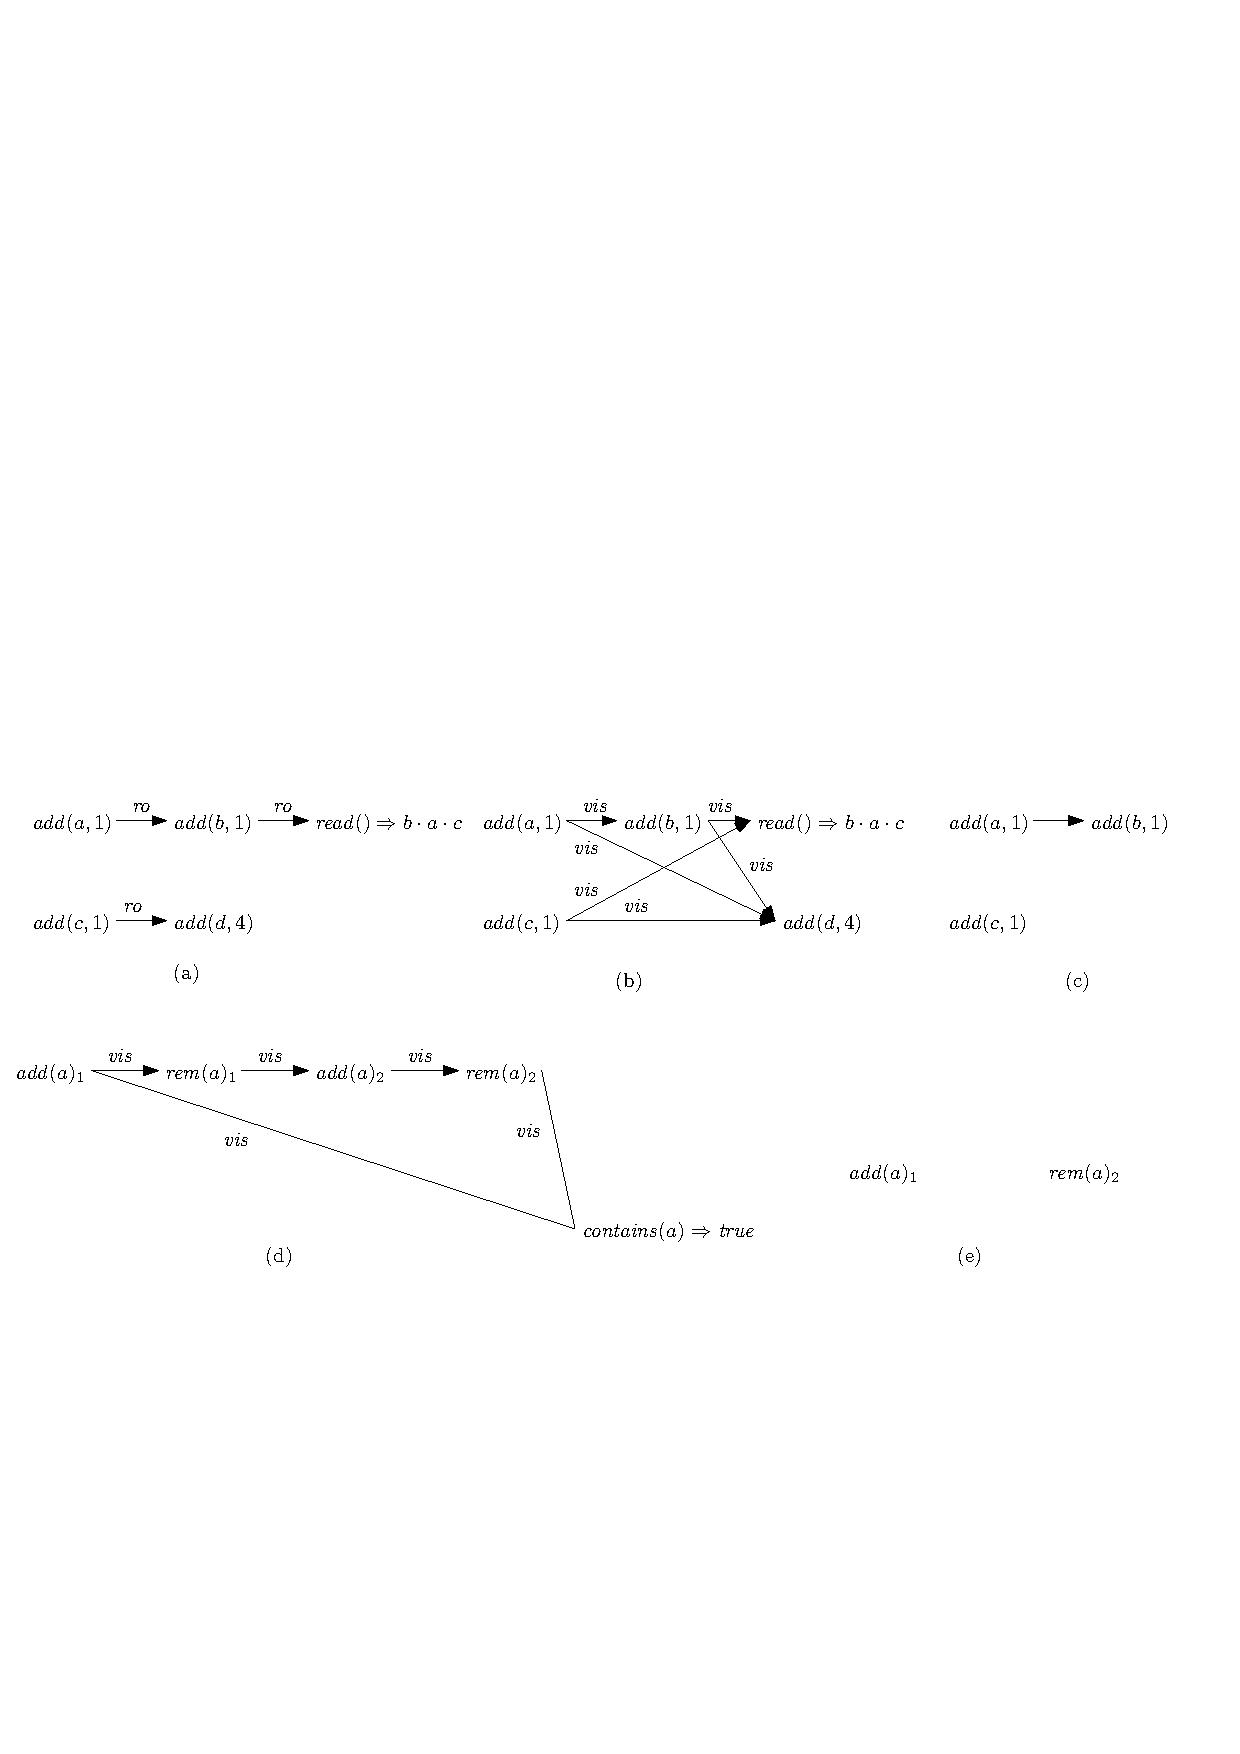
\includegraphics[width=0.75 \textwidth]{figures/PIC-his-anhis-context.pdf}
%\vspace{-10pt}
  \caption{History, its annotated history and operation context. Here $+(a,1)$ represents $\mathit{add}(a,1)$, $r(b \cdot a \cdot c)$ represents $\mathit{read}(b \cdot a \cdot c)$; $+a_1$ and $-a_1$ represents $\mathit{add}(a)$ and $\mathit{rem}(a)$, respectively, while the subscript number is used to distinguish different $\mathit{add(a)}$; $(a,\surd)$ represents $\mathit{contains}(a,\mathit{true})$. In annotated history (b), we use arbitration order $\mathit{add}(b,1) \cdot \mathit{add}(a,1) \cdot \mathit{add}(c,1) \cdot \mathit{add}(d,4)$. Assume that the visibility relation contains the replica order.}
  \label{fig:history, annotated history and operation context}
\end{figure}


{\color {red}Similarly as in \cite{Burckhardt:2014}, in defining specification, we use the notion of operation context, which contains all information necessary to ensure the correctness of an operation.} A operation context of a operation $o$ is a tuple $(O,<,\mathit{arb})$, where $O$ is a set of update operations, $<$ is a relation over $O$, $o \notin O$, and $\mathit{arb}$ is a irreflexive total order over a subset of update operations of $O \cup \{ o \}$. {\color {red}Here we modified that of \cite{Burckhardt:2014} by making $o \notin O$ itself also contained in the arbitration order. This feature is used to deal with list specification.} A specification $\mathit{Spec}$ is a function that maps each operation label $\ell$ into a set of elements, while each of them is a operation context $(O,<,\mathit{arb})$ for some operation $o$ with $\mathit{lab}(o) = \ell$. {\color {red} For example, \figurename~\ref{fig:history, annotated history and operation context} (c) is in specification of $o = \mathit{add}(d,4)$.} A specification is deterministic, if there does not exists query method $m$ and tuple $(O,<,\mathit{arb})$, such that $(O,<,\mathit{arb})$ is in both $\mathit{Spec}(m(a) \Rightarrow b)$ and $\mathit{Spec}(m(a') \Rightarrow b')$, and $a \neq a' \vee b \neq b'$. From now on, we consider only deterministic specifications.

Given an annotated history $(O,\mathit{vis},\mathit{arb})$ and an operation $o \in O$, the operation context of $o$ is a obtained by a tuple $ctxt(o)=(O',<,\mathit{arb}')$, where $O'$ is the set of update operations in $\mathit{vis}^{-1}(o)$, $<$ is the projection of $\mathit{vis}$ over $O'$, and $\mathit{arb}'$ is the projection of $\mathit{arb}$ over update operations of $O' \cup \{ o \}$. Therefore, given an annotated history $(O,\mathit{vis},\mathit{arb})$ and $o_1,o_2 \in O$, if $o_1$ and $o_2$ see the same set of operations, %$\mathit{vis}^{-1}(o_1) = \mathit{vis}^{-1}(o_2)$,
then $O_1 = O_2$ and $<_1 = <_2$, where $ctxt(o_1)=(O_1,<_1,\mathit{arb}_1)$ and $ctxt(o_2)=(O_2,<_2,\mathit{arb}_2)$. This comply with the commutativity intuition of CRDT algorithm. {\color {red} For example, \figurename~\ref{fig:history, annotated history and operation context} (c) is also the operation context of $o = \mathit{add}(d,4)$ in \figurename~\ref{fig:history, annotated history and operation context} (b).} {\color {red}Similarly, this definition modifies that of \cite{Burckhardt:2014} to deal with list.} Note that the uniformly method of obtaining operation context from annotated history is suitable for most specifications. For one special case, the OR-set, we shows how to deal with it in Remark \ref{remark: operation context of OR-set}.

%To comply with the commutativity intuition of CRDT algorithm, we further require that, given an annotated history $(O,\mathit{vis},\mathit{arb})$ and $o_1,o_2 \in O$, if $\mathit{vis}^{-1}(o_1) = \mathit{vis}^{-1}(o_2)$, then $<_1 = <_2$, where $ctxt(o_1)=(O_1,<_1,\mathit{arb}_1)$ and $ctxt(o_2)=(O_2,<_2,\mathit{arb}_2)$.

The notion of Convergent Return-Value Consistency (CRVC, for short) requires that the return value of each operation be correct, and is defined as follows:
%\todo{Define ``an annotated history satisfying SRVC and then a history satisfying SRVC, i.e., there exists $\mathit{vis}$ and $\mathit{arb}$ such that the resulting annotated history satisfies SRVC.}

\begin{definition}[Convergent Return-Value Consistency]
\label{definition:strong return value consistency}
An annotated history $(O,\mathit{vis},\mathit{arb})$ is CRVC w.r.t specification $\mathit{Spec}$, if there exists function $\mathit{ctxt}$, such that,

\begin{itemize}
\setlength{\itemsep}{0.5pt}
\item[-] $\mathit{vis}$ is acyclic.

\item[-] $\forall o \in O$, $\mathit{ctxt}(o) \in Spec(\mathit{lab}(o))$.
\end{itemize}

A history $(O,\mathit{ro})$ is CRVC w.r.t $\mathit{Spec}$, if there exists $\mathit{vis}$ and $\mathit{arb}$, such that $\mathit{ro} \subseteq \mathit{vis}$, and $(O,\mathit{vis},\mathit{arb})$ is CRVC consistent w.r.t $\mathit{Spec}$.
\end{definition}

\noindent {\bf Example 1. OR-set}: Observed-Remove Set (OR-set for short) \cite{Shapiro:2011,Bieniusa:2012} contains four methods: (1) $\mathit{add}(a)$ inserts $a$ into set, (2) $\mathit{rem}(a)$ remove $a$ from set, (3) $\mathit{lookup}(a)\Rightarrow \mathit{true}$ (resp., $\mathit{lookup}(a)\Rightarrow \mathit{false}$) represents that $a$ is in set (resp., $a$ is not in set), and $\mathit{elements}() \Rightarrow S$ represents that the set content is $S$.

%\todo{Why do you need $\top$ as argument ?? If it's because you want to use operation labels for messages as well, I don't like it. Each part of the formalism should be as clear as possible, without unnecessary junk.}

%Let $\Sigma_{\mathit{ORS}} = \{ add(a,\top),rem(\top,a) \vert a \in \mathbb{D} \}$ be the set of contents of update operations.
The specification $S_{\mathit{ORS}}$ is as follows: (1) For $x=\mathit{add}(a)$, $S_{\mathit{ORS}}(x)$ is the set of all tuples $(O,<,\emptyset)$, (2) For $x=\mathit{lookup}(a) \Rightarrow \mathit{true}$ (resp., $x=\mathit{lookup}(a) \Rightarrow \mathit{false}$), $S_{\mathit{ORS}}(x)$ is the set of all tuples $(O,<,\emptyset)$, such that the projection of $<$ over $\mathit{add}(a)$ and $\mathit{rem}(a)$ in $O$ contains a maximal element with operation label $\mathit{add}(a)$ (resp., contains no maximal element with operation label $\mathit{add}(a)$), (3) For $x = \mathit{rem}(a)$, $S_{\mathit{ORS}}(x)$ is the same as $x = \mathit{lookup}(a) \Rightarrow \mathit{true}$, and (4) $S_{\mathit{ORS}}(\mathit{elements}() \Rightarrow S)$ is all the tuples $(O,<,\emptyset)$ that are in $S_{\mathit{ORS}}(\mathit{lookup}(a) \Rightarrow \mathit{true})$ for each $a \in S$, and are in $S_{\mathit{ORS}}(\mathit{lookup}(a)) \Rightarrow \mathit{false}$ for each $a \notin S$. {\color {red} $S_{\mathit{ORS}}$ make $\mathit{rem}$ cancel only $\mathit{add}$ operations ``visible'' to them. For example, \figurename~\ref{fig:history, annotated history and operation context} (e) is in $S_{\mathit{ORS}}(\mathit{lookup}(a) \Rightarrow \mathit{true})$.} 

\noindent {\bf Example 2. Distributed list}: Distributed list has three methods: (1) $\mathit{add}(a,\mathit{pos})$ inserts identifier $a$ into position $\mathit{pos} \in \mathbb{N}$, (2) $\mathit{rem}(a)$ removes the identifier $a$ from list, and (3) $\mathit{read}() \Rightarrow l$ returns the list content. Here intuitively, we assume that each identifier are putted at most once globally. 

%Let $\Sigma_{\mathit{list}} = \{ add(a,pos,\top),rem(\top,a) \vert a \in \mathbb{D},pos \in \mathbb{N} \}$ be the set of contents of update operations.
The specification $S_{\mathit{list}}$ is defined as follows: $(O,<,\mathit{arb}) \in S_{\mathit{list}}(\ell)$, if

\begin{itemize}
\setlength{\itemsep}{0.5pt}
\item[-] %$<^{-1}$ contains finite elements, $<$ is acyclic and 
$arb$ is a total order of $add$ operations in $O \cup \{ o \}$, where $o \notin O$ and is in domain of $arb$.

\item[-] Let $R = \{ i \vert \exists b, (add(b),\_,i),(rem(b),\_,\_) \in O \}$ and $\mathit{seq} = \mathit{arb} \uparrow_{ O \cup \{ o \} \setminus R }$. Then,

    \begin{itemize}
    \setlength{\itemsep}{0.5pt}
    \item[-] Either $\ell = add(a,pos) \wedge \mathit{seq}[pos] = o$,

    \item[-] Or $\ell = rem(a) \wedge (add(a),\_,\_) \in O$,

    \item[-] Or $\ell = read() \Rightarrow l$ and $l$ is obtained by using $\mathit{lab}$ on $\mathit{seq}$. 
    \end{itemize}
\end{itemize}

%\todo{Give a declarative specification of the list, like for OR-set. Descriptions which look like ``imperative programs'', e.g., "We can go through operations", "During this process".}

Where for a relation $R$, $R \uparrow_{S}$ means projection $R$ on $S \times S$. We essentially use the ist order of strong list specification in \cite{Attiya:2016} as the arbitration order. 


\begin{remark}
\label{remark: operation context of OR-set}
For OR-set, the operation context of annotated history is more complicated. {\color {red} For example, given the annotated history \figurename~\ref{fig:history, annotated history and operation context} (d), the operation context of $\mathit{contains}(a,\textit{true})$ in this annotated history should be \figurename~\ref{fig:history, annotated history and operation context} (e), since $-a_2$ does not cancel $+a_1$, and they should not be related.} Formally, given an annotated history $(O,\mathit{vis},\mathit{arb})$ and an operation $o$, $ctxt(o)=(O',<,\mathit{arb}')$, where $O'$ and $\mathit{vis}'$ is as before, and $<$ is defined as $\mathit{vis} \uparrow_{O'} - \{ (o_1,o_2) \vert o_2 \notin \mathit{FstRem}(O,\mathit{vis},o_1),$ $\exists o_3 \in O, (o_1,o_3), (o_3,o_2),(o_1,o_2) \in \mathit{vis}, o_1,o_2 \in O', o_3 \notin O' \}$. {\color {red}Here $\mathit{FstRem}$ records matched $\mathit{add}$ and $\mathit{rem}$ pairs like $(+a_1,-a_1)$,} and is defined as $\mathit{FstRem}(O,\mathit{vis},o) = \{o' \vert \mathit{lab}(o')=\mathit{rem}(a), (o,o') \in \mathit{vis}, \neg \exists o'',  lab(o'') = \mathit{rem}(a)  \wedge (o,o''),(o'',o') \in \mathit{vis} \}$ for $lab(o) = \mathit{add}(a)$.
\end{remark}





%{\color {red}Remark: For OR-set, the operation context of annotated history is more complicated: Given an annotated history $(O,\mathit{vis},\mathit{arb})$ and an operation $o$, $ctxt(o)=(O',<,\mathit{arb}')$, where $O'$ and $\mathit{vis}'$ is as before, and $< = \mathit{vis} \uparrow_{(O' \times O')} - \{ (o_1,o_2) \vert o_2 \notin FstRem(O,\mathit{vis},o_1), \exists o_3 \in O, (o_1,o_3), (o_3,o_2),(o_1,o_2) \in \mathit{vis}, o_1,o_2 \in O', o_3 \notin O' \}$. Here $FstRem(O,\mathit{vis},o)$ is the set of first visible matching remove of $o$ w.r.t $\mathit{vis}$, and is defined as $FstRem(O,\mathit{vis},o) = \{o' \vert lab(o')=rem(a), (o,o') \in \mathit{vis}, \neg \exists o'',  lab(o'') = rem(a)  \wedge (o,o''),(o'',o') \in \mathit{vis} \}$ for $lab(o) = add(a)$.}


%Given an annotated history $(O,\mathit{vis},\mathit{arb})$ and an operation $o$, $ctxt(o)=(O',<,\mathit{arb}')$ of OR-set is defined as follows: $\mathit{arb}' = \emptyset$, and $< = \mathit{vis} \uparrow_{(O' \times O')} - \{ (o_1,o_2) \vert o_2 \notin Minus(O,\mathit{vis},o_1), \exists o_3 \in O, (o_1,o_3), (o_3,o_2),(o_1,o_2) \in \mathit{vis}, o_1,o_2 \in O', o_3 \notin O' \}$. Here $Minus(O,\mathit{vis},o)$ is the set of first visible matching remove of $o$ w.r.t $\mathit{vis}$, and is defined as $Minus(O,\mathit{vis},o) = \{o' \vert lab(o')=rem(a), (o,o') \in \mathit{vis}, \neg \exists o'',  lab(o'') = rem(a)  \wedge (o,o''),(o'',o') \in \mathit{vis} \}$ for $lab(o) = add(a)$.




%The specification $S_{\mathit{list}}$ is defined as follows: $(O,<,arb) \in S_{\mathit{list}}(\ell)$, if

%\begin{itemize}
%\setlength{\itemsep}{0.5pt}
%\item[-] $<^{-1}$ contains finite elements, $<$ is acyclic and $arb$ is a total order of $add$ operations in $O \cup \{ o \}$, where $o \notin O$ and is in domain of $arb$.

%\item[-] {\color {red}Function $f: O \cup \{ o \} \rightarrow P(O \cup \{ o \})$. For the case of $o' \in O$, let $S(o') = f(o_1) \cup \ldots \cup f(o_k)$, where $o_1,\ldots,o_k$ is the immediate predecessor of $o'$ w.r.t $<$. Then, $f(o')$ is recursively defined as

%    \begin{itemize}
%    \setlength{\itemsep}{0.5pt}
%    \item[-] $S(o')$, if $lab(o')=read()\Rightarrow list \wedge list = lab( arb \uparrow_{ (<^{-1}(o')-\{ x \vert (x,\_) \in S(o')\}) } )$.

%    \item[-] $S(o')$, if $lab(o')=add(a,pos) \wedge ( arb \uparrow_{ (<^{-1}(o')-\{ x \vert (x,\_) \in S(o')\}) } )[pos]=o'$.

%    \item[-] $S(o') \cup \{ (o_a,o') \}$, if $lab(o')=rem(pos)\Rightarrow a \wedge ( arb \uparrow_{ (<^{-1}(o')-\{ x \vert (x,\_) \in S(o')\}) } )[pos]=o_a \wedge lab(o_a)=add(a,\_)$.

%    \item[-] $\mathit{Undef}$, otherwise.
%    \end{itemize}

%    For the case of $o$, let $S(o)$ be the union of $f(o'')$ for each $o'' \in O$, and the other part is the same as above. We require that, for each $o' \in O \cup \{ o \}$, $f(o') \neq \mathit{Undef}$.}
%\end{itemize}

%\todo{Give a declarative specification of the list, like for OR-set. Descriptions which look like ``imperative programs'', e.g., "We can go through operations", "During this process".}

%In our definition of distributed list specification, the arbitration order works similarly as the list order of strong list specification in \cite{Attiya:2016}.














%\todo{Use $r$ instead of $rid$ and $i$ instead of $oid$. But be careful to not use $i$ in other contexts, for instance remove the $\forall i$ from the previous section. Keep $i$ and $j$ only for operation ids.}

%CRDT has two kinds of method: query methods and update methods: Operations of query methods take effect only in one replica, while operations of update methods will be delivered to other replicas.

%A specification $Spec$ is a function that maps each operation label $\ell$ into a set of tuples $(O,<,arb)$, where $O$ is a set of update operations, $<$ is a partial order over $O$, and $arb$ is a partial order over $O \cup \{ o \}$ called arbitration order, where $lab(o)=\ell \wedge o \notin O$.

%We require that, given $o_1,o_2 \in O$, if $\mathit{vis}^{-1}(o_1) = \mathit{vis}^{-1}(o_2)$, then $<_1 = <_2$, and $arb_1 \cup arb_2$ is acyclic, where $ctxt(o_1)=(O_1,<_1,arb_1)$ and $ctxt(o_2)=(O_2,<_2,arb_2)$.



%\todo{The rest of the paragraph should be a footnote. Uninteresting details.}
%Here we require that each operation in $O \cup \{ o \}$ has unique operation identifier. Such $(O,<,<_{\mathit{arb}},l)$ tuples are called ($\Sigma$-labeled) partial-ordered set (poset, for short), where $\Sigma$ is a set of update operation contents contains that of $O$. Two labeled posets are isomorphic if there exists a bijection of operations that preserve operation contents, labels and orders. Here we require $Spec$ to be isomorphic closed: if $x \in Spec$ and $x$ and $y$ are isomorphic, then $y \in Spec$. Since the labeling function of poset is fixed, we could ignore it when the context is clear.

%\todo{I would suggest to define specifications only for query operations. I guess that you need to include $o$ in $O$ for the updates like inserting in a list. But this is kind of ugly, so I would prefer that $O$ doesn't contain $o$}

%\todo{I guess $l$ is not needed. An operation is already a label (content in your terms) with ids}

%\todo{Use $\mathit{arb}$ instead of $<_{\mathit{arb}}$. I told you several times, don't try to minimize the space occupied by your notations. And don't use complicated indices or superscripts.}

%\todo{I don't see the "deterministic" condition: for a given tuple $(O,<,arb)$, the return value is unique.}

%\todo{I think that this part about plus-minus specifications is not useful here. Give standard examples and push this discussion/examples when needed.}





%\subsection{Consistencies}
%\label{subsec:consistencies}

%\todo{Define a history as $(O,\mathit{ro})$ (again, forget about long indices), then an annotated history as $(O,\mathit{ro},\mathit{vis},\mathit{arb})$ (dont use $\mathit{mathit}$).}

%A history is a tuple $(O,\mathit{ro})$, where

%\begin{itemize}
%\setlength{\itemsep}{0.5pt}
%\item[-] $O$ is a set of operations.

%\item[-] $\mathit{ro}$ is called the replica order. For each replica $r \in \mathbb{R}$, $\mathit{ro}$ is a irreflexive total order over operations with replica identifier $r$. $\mathit{ro}$ does not relate operations with different replica identifiers. We also require that for each operation $o \in O$, $\mathit{ro}^{-1}(o)$ is finite.
%\end{itemize}

%An annotated history is a tuple $(O,\mathit{ro},\mathit{vis},\mathit{arb})$, where

%\begin{itemize}
%\setlength{\itemsep}{0.5pt}
%\item[-] $(O,\mathit{ro})$ is a history.

%\item[-] $\mathit{vis}$ is irreflexive and acyclic, and is called the visibility order. We require that for each operation $o \in O$, $\mathit{vis}^{-1}(o)$ is finite.

%\item[-] $\mathit{arb}$ is the arbitration order over update operations of $O$.
%\end{itemize}

%\todo{Local interpretation meant something else in our previous paper. Use operation context for $(\mathit{vis}^{-1}(o),<,\mathit{arb}\downarrow (\mathit{vis}^{-1}(o)\times \mathit{vis}^{-1}(o)))$ where $<$ is defined as you say.}

%Given an annotated history $(O,\mathit{ro},\mathit{vis},\mathit{arb})$ and an operation $o \in O$, the operation context of $o$ is a tuple $ctxt(o)=(O_o,<,arb_o)$, where

%\begin{itemize}
%\setlength{\itemsep}{0.5pt}
%\item[-] $O_o$ is the set of update operations in $\mathit{vis}^{-1}(o)$,

%\item[-] $arb_o$ is the projection of $arb$ over update operations of $O_o \cup \{ o \}$.

%\item[-] $< \subseteq <_{\mathit{vis}} \uparrow_{(O_o \times O_o)}$ and it is irreflexive.

%We require that, given operations $o_1,o_2,o'_1,\ldots,o'_m \in O_o$, if $(o_1,o_2) \in \mathit{vis}$ via $o'_1,\ldots,o'_m$, then $(o_1,o_2) \in <$. We say that $(o_1,o_2) \in \mathit{vis}$ via $o'_1,\ldots,o'_m$, if $(o_1,o'_1),$ $(o'_1,o'_2), \ldots, (o'_{\mathit{m-1}},o'_m),(o'_m,o_2)$ are all in $\mathit{vis}$.

%\item[-] {\color {red}We require that, given $o_1,o_2 \in O$, if $\mathit{vis}^{-1}(o_1) = \mathit{vis}^{-1}(o_2)$, then $<_1 = <_2$, and $arb_1 \cup arb_2$ is acyclic, where $ctxt(o_1)=(O_1,<_1,arb_1)$ and $ctxt(o_2)=(O_2,<_2,arb_2)$.}
%\end{itemize}

%Let us define strong-return-value consistency (SRVC consistency, for short) as follows:

%\todo{Define ``an annotated history satisfying SRVC and then a history satisfying SRVC, i.e., there exists $\mathit{vis}$ and $\mathit{arb}$ such that the resulting annotated history satisfies SRVC.}

%\begin{definition}[Strong-return-value consistency]
%\label{definition:strong return value consistency}
%An annotated history $(O,\mathit{ro},\mathit{vis},\mathit{arb})$ is SRVC w.r.t specification $Spec$, if there exists function $ctxt$, such that,

%\begin{itemize}
%\setlength{\itemsep}{0.5pt}
%\item[-] $\mathit{ro} \subseteq \mathit{vis} \wedge \mathit{vis}$ is acyclic.

%\item[-] $\forall o \in O$, $ctxt(o) \in Spec(lab(o))$.
%\end{itemize}

%A history $(O,\mathit{ro})$ is SRVC w.r.t $Spec$, if there exists $\mathit{vis}$ and $\mathit{arb}$, such that $(O,\mathit{ro},\mathit{vis},\mathit{arb})$ is SRVC consistent w.r.t $Spec$.
%\end{definition}
















%!TEX root = draft.tex

\section{Reference Implementation}
\label{sec:reference implementation}

%In this section, we propose an abstract implementation called reference implementation, which will be used as specification in simulation proof of later section.

We present a generic definition of CRDT reference implementations as labeled transition systems. This definition is parametrized by a specification $Spec$ defining the abstract semantics of the CRDT's operations.
%sec:specifications and consistencies

A labeled transition system (LTS, for short) is a tuple $A = (Q,\Sigma,\rightarrow,q_0)$, where $Q$ is a set of states, $\Sigma$ is an alphabet of transition labels, $\rightarrow \subseteq Q \times \Sigma \times Q$ is a transition relation and $q_0$ is the initial state. An execution of $A$ is defined as usual by a sequence of transitions starting from the initial state $q_0$. A trace is the sequence of transition labels from an execution. We say that $A$ is deterministic, if for each state $q$ and each transition label $\alpha$, $q$ has at most one $\rightarrow$ successor with transition label $\alpha$.


\begin{figure}[t]
  \centering
  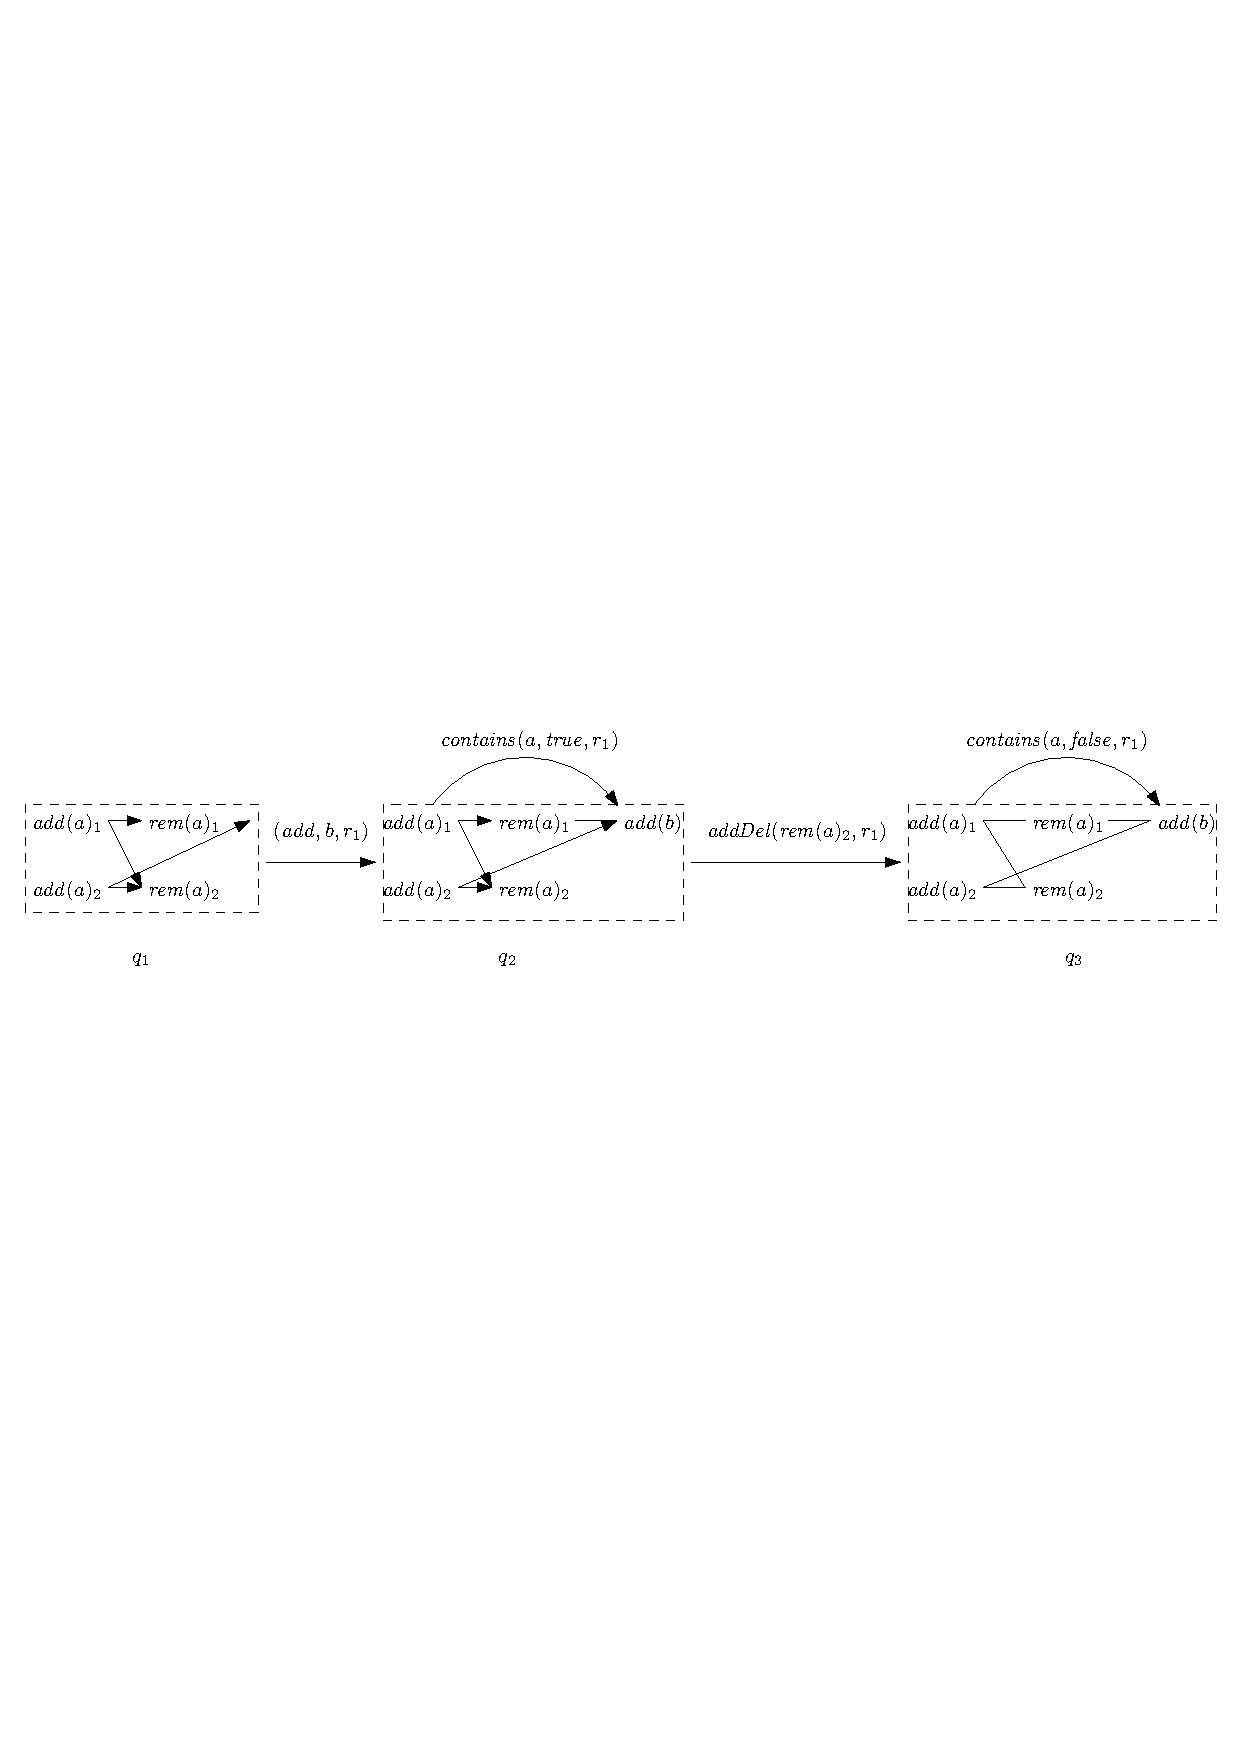
\includegraphics[width=1 \textwidth]{figures/PIC-RImp.pdf}
%\vspace{-10pt}
  \caption{Reference implementation for OR-set. Arrow of same replica represents replica order, while arrow between different replica represents delivery order.}
  \label{fig:reference implementation for OR-set}
\end{figure}

Each state of the reference implementation is a history, which for succinctness, contains only update operations, together with an arbitration order (which has the same meaning as in annotated histories) and a \emph{delivery} relation $del$ which is a ``more succinct'' substitute of the visibility relation: for two operations $o_1$ and $o_2$ submitted at replicas $r_1$ and $r_2$, respectively, $del(o_1,o_2)$ denotes the fact that $o_2$ is the first operation submitted to $r_2$ after the operation $o_1$ is delivered to $r_2$. We write $del(o_1,r_2)$ when $o_1$ is delivered after the last operation submitted to $r_2$. For instance, consider the execution fragment depicted in \figurename~\ref{fig:reference implementation for OR-set} (this is extracted from a reference implementation of the OR-set). In state $q_1$, $(add(a)_2,r_1) \in \mathit{del}$ (denoted by the edge going to the end of the replica $r_1$) means that the effect of $add(a)_2$ is delivered to replica $r_1$ after all the operations submitted at $r_1$ ($add(a)_1$ and $rem(a)_1$) happened, while $(add(a)_1,rem(a)_2) \in \mathit{del}$ means that the effect of $add(a)_1$ is delivered to replica $r_2$ at a time point earlier than when $rem(a)_2$ is submitted and later than when $add(a)_2$ is submitted. The visibility relation can be obtained as the union of $\mathit{ro}$ and the composition of $\mathit{del}$ with $\mathit{ro}$. The reference implementation has two kinds of transitions: transitions labeled by operations which may increase the history and possibly the arbitration order (query operations leave the history stored in the state unchanged) and transitions labeled by $\mathit{addDel}(\_,\_)$ which increase the delivery relation. A transition labeled by an $\ell$ operation submitted to replica $r$ is enabled when the operation context at the newest time-point of replica $r$ is in $\mathit{Spec}(\ell)$. An example of such a transition is the one from $q_1$ to $q_2$ in \figurename~\ref{fig:reference implementation for OR-set} or the self-loops in $q_2$ and $q_3$. The transition from $q_2$ to $q_3$ is an example of a transition that increases the delivery relation. Such transitions make the reference implementation deterministic.

%%We introduce a new relation $\mathit{del}$ called delivery relation to capture the intuition that CRDT only broadcast effect of one operation.
%
%%Since CRDTs normally does not use speculative execution, the annotated history increase monotonously during transitions of $\mathit{Spec}$.
%
%
%{\color {red}Let us use the example of \figurename~\ref{fig:reference implementation for OR-set} to explain how to model specification $\mathit{Spec}$ as a deterministic LTS $\mathit{RImp}(\mathit{Spec})$.
%
%\begin{itemize}
%\setlength{\itemsep}{0.5pt}
%\item[-] Each state of $\mathit{Spec}$ is an annotated history. Since CRDT normally does not use speculative execution, the annotated history increase monotonously during transitions of $\mathit{Spec}$. For simplicity these annotated history only contains update operations. We introduce a new relation $\mathit{del}$ called delivery relation to capture the intuition that CRDT only broadcast effect of one operation.
%
%
%\item[-] To do a $\ell$ operation on replica $r$, we check whether the operation context of the newest time-point of replica $r$ is in $\mathit{Spec}(\ell)$. If $\ell$ is query, then we have a loop transition, as the self-loop of $q_2$ in \figurename~\ref{fig:reference implementation for OR-set}; if $\ell$ is update, we increasing the annotated history by put a $\ell$ operation in the newest time-point of replica $r$, as the transition from $q_1$ to $q_2$ in \figurename~\ref{fig:reference implementation for OR-set}.
%
%\item[-] To make LTS be deterministic, we make the event of when a operation becomes visible to a replica also transition label. For example, the transition from $q_2$ to $q_3$ in \figurename~\ref{fig:reference implementation for OR-set} represents that $-a_2$ begins to be visible to replica $r_1$. Thus, every change to visibility relation is explicitly.
%\end{itemize} }

Formally, the reference implementation $\mathit{RImp}(\mathit{Spec}) = (Q,\Sigma,\rightarrow,q_0)$ is constructed as follows:

%\todo{Again, what is the purpose of $\mathit{li}$ and $correct$ ? The implementation should be a transition system like in the first section. No additional elements in the tuples.}

\begin{itemize}
\setlength{\itemsep}{0.5pt}
\item[-] Each state $(O,\mathit{ro},\mathit{del},\mathit{arb}) \in Q$ contains four tuples: $O$ is a set of update operations, $\mathit{ro}$ is the replica order, $\mathit{del} \subseteq (O \times O) \cup (O \times \mathbb{R})$ is the delivery relation, and $\mathit{arb}$ is the arbitration order.

%Each state of $Q$ records the set of updates already executed, when they were delivered to the different replicas, and the arbitration order.

    %Each state $(O,\mathit{ro},\mathit{del},\mathit{arb}) \in Q$ contains four tuples: $O$ is a set of update operations where each operation in $O$ has unique operation identifier; $\mathit{ro}$ is the replica order and $(O,\mathit{ro})$ a history; $\mathit{del} \subseteq (O \times O) \cup (O \times \mathbb{R})$ is a relation that records operation delivery and is called deliver order. {\color {red}Assume $o_2$ happens in replica $r_2$. $(o_1,o_2) \in \mathit{del}$ represents that the time point of delivering the effect of $o_1$ to replica $r_2$ is after all operations of replica $r_2$ that happens earlier than $o_2$, and before the time point  $o_2$ happens}. $(o,r) \in \mathit{del}$ represents that the effect of $o$ is delivered to replica $r$ after the time point of the last operation of replica $r$. we require $\mathit{del}$ to only relate operations with different replica identifier; $\mathit{arb} \subseteq O \times O$ is the arbitration order.
%\todo{$vis$ shouldn't be in the state.}

%\item[-] $\Sigma$ contains two kinds of transition labels: The first is operation labels tagged with replica identifier and arbitration order, in the form $(m,a,b,r,\mathit{arb})$, where $m \in \mathbb{M}, a,b \in \mathbb{D}, r \in \mathbb{R}$, and $arb \subseteq O \times O$; The second kind is events representing the points in time where operations are delivered, in the form $addDel(o,r)$, where $o \in \mathbb{O}, r \in \mathbb{R}$.


%\item[-] $\Sigma$ contains two kinds of transition labels: The first is operation labels tagged with replica identifier and modification of arbitration order, in the form $(m,a,b,r,ind)$, where $m \in \mathbb{M}, a,b \in \mathbb{D}, r \in \mathbb{R}$, and $ind \in \mathbb{N}$. Here $ind = 0$ means that the arbitration order does not change, while $ind >0$ means that the arbitration order is changed by inserting the newly generated operations into $ind$-th position; The second kind is events representing the points in time where operations are delivered, in the form $addDel(o,r)$, where $o \in \mathbb{O}, r \in \mathbb{R}$.

\item[-] $\Sigma$ contains two kinds of transition labels: $m(a,b,r,\mathit{arb})$ which represents the fact that an $m(a) \Rightarrow b$ operation is submitted at replica $r$ and the arbitration order is changed into $\mathit{arb}$ (the reason of using $\mathit{arb}$ in the transition label is to make $\mathit{RImp}(\mathit{Spec})$ deterministic) and $\mathit{addDel}(o,r)$ which represents the fact that operation $o$ begins to be visible to replica $r$. The transition label $m(a,b,r,\mathit{arb})$ could be simplified by giving just the index of this operation in the arbitration order instead of the full arbitration. We prefer this version to simplify the technical exposition.

%$\Sigma$ contains two kinds of transition labels: The first is operation labels tagged with replica identifier and arbitration order, in the form $(m,a,b,r,\mathit{arb})$, where $m \in \mathbb{M}, a,b \in \mathbb{D}, r \in \mathbb{R}$, and $\mathit{arb}$ is the arbitration order. The second kind is events representing the points in time where operations are delivered, in the form $addDel(o,r)$, where $o \in \mathbb{O}, r \in \mathbb{R}$.

\item[-] $\rightarrow \subseteq Q \times \Sigma \times Q$ is the transition relation. The transition rules of $\rightarrow$ can be found in \figurename~\ref{fig:transition rules of RImpSpec}, and related notions are defined as follows:


    \begin {itemize}

%    \item[-] the visibility relation $\mathit{vis}=(\mathit{del}\circ\mathit{ro})\cup\mathit{ro}$

    \item[-] $\mathit{visTo}(O,r,\mathit{del}) = \mathit{ro}|_r\cup \{ \mathit{del}^{-1}(o) \vert o \in \mathit{ro}|_r \} $ is the set of operations that are currently visible to replica $r$.
    %Here we require $\mathit{vis}$ to be acyclic and irreflexive, and $\mathit{vis}^{-1}$ to be finite.

    %Let $\mathit{vis} = \mathit{del} \cdot \mathit{ro}$ be the visibility relation. We further require $\mathit{vis}$ to be acyclic and irreflexive, and $\mathit{vis}^{-1}$ to be finite. Let $visTo(O,r,\mathit{vis}) = \{ vis^{-1}(o') \vert o'=(\_,r,\_) \in O \} \cup (vis^{-1}(r))$ be the set of operations that are visible to newest time point of replica $r$ or some operations of replica $r$.

    \item[-] %{\color {red}$f_{\mathit{ctxt}}$ is a function that generate possible operation contexts if $o$ is done. It needs to guess new arbitration relation if necessary:}
      given $q = (O,\mathit{ro},\mathit{del},\mathit{arb})$ and $o=(\_,r,\_) \notin O$, ${\mathit{ctxt}}(q,o)$ returns the potential operation context of $o$ in a state reached from $q$ by an $o$ labeled transition, i.e., a tuple $(O',\mathit{vis}',\mathit{arb}')$, where $O' = \mathit{visTo}(O,r,\mathit{del})$, $\mathit{vis}'$ is the projection of $\mathit{vis}=(\mathit{del}\circ\mathit{ro})\cup\mathit{ro}$ on $O'$, and $\mathit{arb}'$ is the projection of $\mathit{arb}$ on $O'$.

        %\begin{itemize}
        %\setlength{\itemsep}{0.5pt}
        %\item[-] $O' = visTo(O,r,\mathit{vis}) \cup \{ o \}$.

        %\item[-] $\mathit{vis'} = \mathit{vis} \uparrow_{(O' \times O')} \cup \{ (o',o) \vert (o',r) \in \mathit{vis} \}$.

        %\item[-] If $o$ is an update operation, then $\mathit{arb}'$ is obtained from $\mathit{arb} \uparrow_{(O' \times O')}$ by possibly adding relations between $O'$ and $\{ o \}$; Else, $\mathit{arb}' = \mathit{arb} \uparrow_{(O' \times O')}$.
        %\item[-] $\mathit{arb}'$ is obtained from $\mathit{arb} \uparrow_{(O' \times O')}$ by possibly insert update operation $o$ into some place.
        %\end{itemize}

    %\item[-] $f_{\mathit{ar}}(\mathit{arb},o)$ returns an arbitration order that is obtained from $\mathit{arb}$ by possibly adding relations between $O$ and $\{ o \}$.
%    \item[-] {\color {red}$\mathit{rand}(\mathit{arb},o)$ randomly returns an arbitration order that is obtained from $\mathit{arb}$ by either do nothing or insert update $o$ into some place.}

    \item[-] $\mathit{ro} \oplus o = ro \cup \{ (o',o) \vert o' = (\_,r,\_) \in O \}$ and $\mathit{del} \oplus o$ returns a new delivery relation obtained from $del$ by transforming each $(o',r)$ into $(o',o)$.

    \item[-] $\mathit{arb}\oplus o$ denotes all the arbitration orders obtained by inserting $o$ in the total order represented by $\mathit{arb}$.

    %\item[-] $pos(l,a)$ returns the position of $a$ in list $l$.
    \end{itemize}
Note that, for simplicity, query operations don't modify the arbitration order.
%    {\color {red}Note that the arbitration order may be changed only when new operation happens, while delivery does not change arbitration order.}

\item[-] $q_0=(\emptyset,\emptyset,\emptyset,\emptyset)$ is the initial state.
\end{itemize}

\begin{figure}[ht]
Transitions increasing the delivery relation:
\[
\begin{array}{l c}
\bigfrac{ o \in O\quad (o,r)\notin visTo(O,r,\mathit{del}) }
{ (O,\mathit{ro},\mathit{del},\mathit{arb}) {\xrightarrow{addDel(o,r)}} (O,\mathit{ro},\mathit{del} \cup \{ (o,r) \},\mathit{arb}) } %{\mathit{Delivery}}
\end{array}
\]


%\[
%\begin{array}{l c}
%\bigfrac{ o=(\ell,r,\_) \notin O, \exists x, x \in f_{\mathit{ctxt}}((O,\mathit{ro},\mathit{del},\mathit{arb}),o) \wedge x \in Spec(\ell) }
%{ (O,\mathit{ro},\mathit{del},\mathit{arb}) {\xrightarrow{m(a,b,r,\mathit{arb})}} (O,\mathit{ro},\mathit{del},\mathit{arb}) } {\mathit{Query}}
%\end{array}
%\]
Transitions for submitting query operations:
\[
\begin{array}{l c}
\bigfrac{ m \in \mathbb{Q}\quad \ell = m(a) \Rightarrow b\quad o=(\ell,r,\_) \notin O\quad {\mathit{ctxt}}((O,\mathit{ro},\mathit{del},\mathit{arb}),o) \in Spec(\ell) }
{ (O,\mathit{ro},\mathit{del},\mathit{arb}) {\xrightarrow{m(a,b,r,\emptyset)}} (O,\mathit{ro},\mathit{del},\mathit{arb}) } %{\mathit{Query}}
\end{array}
\]


%\[
%\begin{array}{l c}
%\bigfrac{ o = (\ell,r,\_) \notin O, \exists x, x = (O',\_,f_{\mathit{ar}}(\mathit{arb},o) \uparrow_{O'} ) \in f_{\mathit{ctxt}}((O,\mathit{ro},\mathit{del},\mathit{arb}),o) \wedge x \in %Spec(\ell) }
%{ (O,\mathit{ro},\mathit{del},\mathit{arb}) {\xrightarrow{m(a,b,r,f_{\mathit{ar}}(\mathit{arb},o))}} (O \cup \{ o \},\mathit{ro} \oplus o ,\mathit{del} \oplus %o,f_{\mathit{ar}}(\mathit{arb},o)) } {\mathit{Update}}
%\end{array}
%\]
Transitions for submitting updates:
\[
\begin{array}{l c}
\bigfrac{ 
\begin{array}{c}
 m \in \mathbb{U}\quad \ell = m(a) \Rightarrow b\\
o = (\ell,r,\_) \notin O\quad \mathit{arb}'\in \{\mathit{arb}\}\cup \mathit{arb}\oplus o
\quad
  {\mathit{ctxt}}((O,\mathit{ro},\mathit{del},\mathit{arb}'),o) \in Spec(\ell) 
\end{array}
  }
{ (O,\mathit{ro},\mathit{del},\mathit{arb}) {\xrightarrow{m(a,b,r,\mathit{arb}')}} (O \cup \{ o \},\mathit{ro} \oplus o ,\mathit{del} \oplus o,\mathit{arb}') } %{\mathit{Update}}
\end{array}
\]

\caption{Transition rules of $\rightarrow$}
\label{fig:transition rules of RImpSpec}
\end{figure}

%\FloatBarrier
The reference implementation corresponding to the OR-set specification in Example~\ref{} is obtained as an instantiation of the above definition where even for update operations ($\mathit{add}$ and $\mathit{rem}$) the arbitration order contained in transition labels is $\emptyset$. Similarly, for the list specification in Example~\ref{}, only the transition labels corresponding to $\mathit{add}$ operations contain a non-empty arbitration order.

%
%
%
%\begin{itemize}
%\setlength{\itemsep}{0.5pt}
%\item[-] {\color {red}For OR-set, $f_{\mathit{ctxt}}$ and $\mathit{rand}(\mathit{arb},o)$ uses only arbitration order $\emptyset$.}
%
%\item[-] For distributed list: In $f_{\mathit{ctxt}}$, $\mathit{arb}'$ is obtained from $\mathit{arb} \uparrow_{O'}$ by inserting $o$ into some place if $o$ is a $add$ operation, or unchanged otherwise. $\mathit{rand}(\mathit{arb},o)$ returns an arbitration order that is obtained from $\mathit{arb}$ by insert $o$ into some place if $o$ is a $add$ operation, or unchanged otherwise.
%\end{itemize}

Assuming deterministic specifications $\mathit{Spec}$ and that the operation identifier generation is deterministic, the reference implementation $\mathit{RImp}(\mathit{Spec})$ is itself deterministic.
The annotated history $(O,\mathit{ro},\mathit{vis},\mathit{arb})$ corresponding to an execution $q_0 {\xrightarrow{\alpha_1}} q_1 \ldots$ of $\mathit{RImp}(\mathit{Spec})$ can be defined as expected: $O$ is the set of operations included in transition labels, $\mathit{vis}$ is defined from replica order and the delivery relation, and $\mathit{arb}$ is the union of the arbitration orders included in each $q_i$. A history $(O,\mathit{ro})$ can be extracted from an execution in a similar way. Let $\mathit{his}(\mathit{RImp}(\mathit{Spec}))$ be the set of histories corresponding to executions of $\mathit{RImp}(\mathit{Spec})$. The following result shows that any (annotated) history generated by $\mathit{RImp}(\mathit{Spec})$ satisfies CRVC (see Appendix \ref{sec:appendix definitions and proofs of section reference implementation}).

\begin{theorem}
\label{theorem:histories of reference implementation are SRV consistent}
For each $h \in \mathit{his}(\mathit{RImp}(\mathit{Spec}))$, $h$ is CRVC w.r.t $\mathit{Spec}$.
\end{theorem}

\noindent
{\bf Causal delivery.} The reference implementations defined above can be constrained so that operation delivery is consistent with the causal order between operations.
Given a state $q = (O,\mathit{ro},\mathit{del},\mathit{arb})$, an operation $o_1\in O$ \emph{happens-before} an operation $o_2\in O$, denoted by $o_1 <_{\mathit{hb}} o_2$, if $(o_1,o_2) \in (\mathit{ro}\cup \mathit{del})^*$. A state of the reference implementation satisfies \emph{causal delivery} if for each pair of update operations $(o_1,o_2)$ in this state such that $o_1 <_{\mathit{hb}} o_2$, $o_2$ is delivered to replica $r$ only when $o_1$ has already been delivered to replica $r$. For example, the state $q_3$ in \figurename~\ref{fig:reference implementation for OR-set} satisfies causal delivery, e.g., $add(a)_2 <_{\mathit{hb}} rem(a)_2$ and $add(a)_2$ has already been delivered to replica $r_1$ when $rem(a)_2$ is delivered to $r_1$.

To abstract CRDT implementations that assume causal delivery of messages (which can be defined as for operations), we use a class of reference implementations $\mathit{RImp}(\mathit{Spec})_{\mathit{cd}}$ where operations are delivered in the causal order. Formally, this consists in strengthening the transition rule corresponding to delivery events as follows:

%The reference implementation with causal delivery of $Spec$ is given as an LTS $RImp(Spec)_{\mathit{cd}} = (Q,\Sigma,q_0,\rightarrow)$. $RImp_{\mathit{cd}}(Spec)$ can be obtained from $RImp(Spec)$ by only changing the transition rules of delivery into the following:

\medskip
%\setlength{\itemsep}{0.5pt}
$\begin{array}{l c} \bigfrac{o \in O\quad o\mbox{ is minimal w.r.t $<_{\mathit{hb}}$ in }\{ o' \vert o' \in O \wedge o' \notin \mathit{visTo}(O,r,\mathit{del}) \}} {(O,\mathit{ro},\mathit{del},\mathit{arb}) {\xrightarrow{addDel(o,r)}} (O,\mathit{ro},\mathit{del} \cup \{ (o,r) \},\mathit{arb})} \end{array}$

%The following lemma states that $RImp(Spec)_{\mathit{cd}}$ contains all the traces of $RImp(Spec)$ that are causal delivery. Its proof can be found in Appendix \ref{sec:appendix definitions and proofs of section reference implementation}.

%\begin{lemma}
%\label{lemma:RImpcdSpec contains all the sequences of RImpSpec that are causal delivery}
%$\llbracket RImp(Spec)_{\mathit{cd}} \rrbracket = \{ t \vert t \in \llbracket RImp(Spec) \rrbracket \wedge t$ satisfies causal delivery $\}$.
%\end{lemma}




\forget{
\noindent {\bf Example 3. $RImp(S_{\mathit{ORS}})$}: function $ctxt$ and predicate $cor$ are defined as follows:
\begin{itemize}
\setlength{\itemsep}{0.5pt}
\item[-] Given $o=(\_,r,\_)$ and $q=(O,ro,del,\emptyset)$, $ctxt(q,o) = (visTo(O,r,vis),<_1,\emptyset)$, where $<_1 = vis \uparrow_{(O_1 \times O_1)} - \{ (o_1,o_2) \vert o_2 \notin Minus(q,o_1), \exists o_3, o_1 {\xrightarrow{vis}} o_3 {\xrightarrow{vis}} o_2, o_1,o_2 \in visTo(O,r,vis), o_3 \notin visTo(O,r,vis) \}$.

Here $Minus(q,o_1)$ is defined as follows: (1) if $lab(o_1)=add(a)$, then $Minus(q,o_1) = \{o_2 \vert lab(o_2)=rem(a), o_1 {\xrightarrow{vis}} o_2, \neg \exists o_3, ( lab(o_3) = rem(a) ) \wedge ( o_1 {\xrightarrow{vis}} o_3 {\xrightarrow{vis}} o_2 ) \}$, (2) otherwise, $Minus(q,o_1) = \emptyset$.

\item[-] $cor((O,ro,del,arb))$ holds, if

    \begin{itemize}
    \setlength{\itemsep}{0.5pt}
    \item[-] $arb= \emptyset$.

    \item[-] $\forall o \in O$, if $lab(o)=rem(a)$, then $\exists o', o \in Minus(q,o')$.
    \end{itemize}
\end{itemize}

\noindent {\bf Example 4. $RImp(S_{\mathit{list}})$}: function $ctxt$ and predicate $cor$ are defined as follows:

\begin{itemize}
\setlength{\itemsep}{0.5pt}
\item[-] Given $q = (O,ro,del,arb)$ and $o =(\_,r,\_)$, $ctxt(q,o) = ( O_1 ,<_1, arb_1 )$, where $O_1 = visTo(O,r,vis)$, $<_1 = vis \uparrow_{(O_1 \times O_1)}$, and $arb_1$ is as follows: (1) if $lab(o)=add(\_)$, then $arb_1$ is a total order generated by adding $o$ into some place of $arb$, (2) otherwise, $arb_1 = arb$. We also require that

\item[-] $cor((O,ro,del,arb))$ holds, if

    \begin{itemize}
    \setlength{\itemsep}{0.5pt}
    \item[-] $arb$ is a acyclic and irreflexive total order over $add$ operations of $O$.

    \item[-] For each operation $o \in O$, $f(o) \neq \mathit{Undef}$.
    \end{itemize}
\end{itemize}
}


















%%% Local Variables:
%%% mode: latex
%%% TeX-master: "draft"
%%% End:


%!TEX root = draft.tex

\section{Implementation}
\label{sec:implementation}

{\color {red}In CRDT algorithm, each replica has a local state. When a replica do a operation, it is done locally without synchronization with other replica. If this is an update operation, then this replica will broadcast a message to all other replicas.} Let $\mathbb{L}$ be the set of local state, and $\mathbb{MSG}$ be the set of messages. Each message is of the form $(d,r_s,r_d)$ where $r_s \in \mathbb{R}$ is the identifier of replica that generates this message, and $r_d \in \mathbb{R}$ is the destination replica identifier of this message. A CRDT implementation $\mathit{imp}$ is defined as a tuple $(\rightarrow_o,\rightarrow_m,d_0,f_{\mathit{arb}}, \Sigma_e)$, where

\begin{itemize}
\setlength{\itemsep}{0.5pt}
\item[-] $\rightarrow_o: \mathbb{L} \times \mathbb{M} \times \mathbb{D} \times \mathbb{R} \rightarrow \mathbb{L} \times \mathbb{D} \times \mathit{Pow}(\mathbb{MSG})$ shows how method update local state and generate messages. $(d,m,a,r) \rightarrow_o (d',b,\mathit{msgs})$ represents that, when the local state of replica $r$ is $d$, if we call method $m$ with argument $a$ in replica $r$, then we obtain return value $b$, change the local state of replica $r$ into $d'$, and generate a set $\mathit{msgs}$ of messages. Here $\mathit{Pow}(\mathbb{MSG})$ is the power set of $\mathbb{MSG}$. If $m \in \mathbb{U}$, then $\mathit{msgs} = \{ (x,r,r') \vert r' \in \mathbb{R} \wedge r \neq r' \}$ for some $x$. Otherwise, $\mathit{msgs} = \emptyset$. {\color {red}The violation of pre-condition of method is modeled by mapping to $\mathit{undef}$.}

\item[-] $\rightarrow_m: \mathbb{L} \times \mathbb{R} \times \mathbb{MSG} \rightarrow \mathbb{L}$. $(d,r,\mathit{msg}) \rightarrow_m d'$ represents that, if the local state of replica $r$ is $d$ and we apply message $\mathit{msg}$, then we obtain local state $d'$. {\color {red}The violation of pre-condition of applying a message is modeled by mapping to $\mathit{undef}$.}

\item[-] $d_0 \in \mathbb{L}$ is the initial local state.

\item[-] $f_{\mathit{arb}}$ takes the local states of each replica, and a set of messages as arguments, and returns a total order over elements, while each element represents an operation. Let $\Sigma_e$ be the set of such elements.

    %To do this, we need a method to extract elements from local states and messages. Let the set of extracted elements to be $\Sigma_e$.

%\item[-] $f_{o}: \Sigma_{\mathtt{RD}}^{\vert \mathbb{R} \vert} \times Pow(\mathbb{MSG}) \Rightarrow Pow(\Sigma_o)$, where $\Sigma_o$ is a set of elements and each element represents an operation. Given replica data of each replica, $f_{o}$ is used to obtain the ``operations'' known by current state of implementation.

%\item[-] $f_{arb}: \Sigma_{\mathtt{RD}}^{\vert \mathbb{R} \vert} \times Pow(\mathbb{MSG}) \Rightarrow \Sigma_o^*$. Given replica data of each replica and messages, $f_{arb}$ is used to obtain the arbitration relation.
\end{itemize}


The semantics of $\mathit{imp}$ is given as an LTS $\mathit{Sem}(\mathit{imp}) = (Q,\Sigma,\rightarrow,q_0)$, where

\begin{itemize}
\setlength{\itemsep}{0.5pt}
\item[-] Each state $(\mathit{data},\mathit{msgs}) \in Q$ contains two tuples: $\mathit{data}: \mathbb{R} \rightarrow \mathbb{L}$ is the local state of each replica, $\mathit{msgs} \subseteq \mathbb{MSG}$ is the set of messages that are waiting to be applied.

\item[-] $\Sigma$ contains two kinds of transition labels. $m(a,b,r,\mathit{arb})$ represents that a $m(a) \Rightarrow b$ operation is done in replica $r$ and the arbitration order is changed into $\mathit{arb}$. $\mathit{apply}(\mathit{msg})$ represents applying message $\mathit{msg}$.

\item[-] $\rightarrow$ is the transition relation and is defined as follows:

    \begin{itemize}
    \setlength{\itemsep}{0.5pt}
    \item[-] %{\color {red}When doing operations, we keep messages unique.}

    $\begin{array}{l c} \bigfrac{ (\mathit{data}[r],m,a,r) \rightarrow_o (d,b,\mathit{msgs}'), \mathit{msg} \cap \mathit{msgs}' = \emptyset, f_{\mathit{arb}}((\mathit{data}[r:d], \mathit{msgs} \cup \mathit{msgs}')) = \mathit{arb}} {(\mathit{data},\mathit{msgs}) {\xrightarrow{(m,a,b,r,\mathit{arb})}} (\mathit{data}[r:d], \mathit{msgs} \cup \mathit{msgs}')} \end{array}$

    \item[-] {\color {red} When a message is applied, we remove it from $\mathit{msgs}$.}

    $\begin{array}{l c} \bigfrac{ \mathit{msg} = (\_,\_,r) \in \mathit{msgs},(\mathit{data}[r],r,\mathit{msg}) \rightarrow_m d } {(\mathit{data},\mathit{msgs}) {\xrightarrow{\mathit{apply}(\mathit{msg})}} (\mathit{data}[r:d],\mathit{msgs} - \{ \mathit{msg} \})} \end{array}$
    \end{itemize}

\item[-] $q_0 = (data_0,\emptyset)$ is the initial state, where $data_0$ maps each replica identifier into $d_0$.
\end{itemize}

An trace of $\mathit{imp}$ satisfies causal delivery, if given $o_1 <_{\mathit{hb}} o_2$, then we can apply message generated by $o_2$ on a replica, if the message generated by $o_1$ has already been applied on this replica. The semantics of $\mathit{imp}$ with causal delivery is given as an LTS $\mathit{Sem}(\mathit{imp})_{\mathit{cd}}$, and we give its detailed definition in Appendix \ref{sec:appendix definitions and proofs of section implementation}. Each state of $\mathit{Sem}(\mathit{imp})_{\mathit{cd}}$ is a tuple $(\mathit{data},\mathit{msgs},\mathit{msghb})$. {\color {red}Here $\mathit{msghb}$ record the happen-before relation between messages with same destination replica, and we can only apply a minimal messages of $\mathit{msgs}$ w.r.t $\mathit{msghb}$.}




\noindent {\bf Example 6. OR-set algorithms of \cite{Shapiro:2011}}: This algorithm assumes causal delivery. Its tuple are as follows:

{\color {red}
\begin{itemize}
\setlength{\itemsep}{0.5pt}
\item[-] $\mathbb{L} = \{ (S,\mathit{ctr}) \vert S \subseteq \mathbb{D} \times (\mathbb{R} \times \mathbb{N}), \mathit{ctr} \in \mathbb{N} \}$. Elements of $S$ are of form $(a,id)$, and $\mathit{ctr}$ is per-replica counter to make $id$ unique.

\item[-] $(S,\mathit{ctr}) \xrightarrow[\mathit{msgs} = \{ (a,\mathit{id},r,r') \vert r' \neq r \}]{(\mathit{add},a,r)}_o (S \cup \{ (a,\mathit{id}) \}, \mathit{ctr}+1)$ and $\mathit{id} = (r,\mathit{ctr})$.

\item[-] $(S,\mathit{ctr}) \xrightarrow[\mathit{msgs} = \{ (a,S'',r,r') \vert r' \neq r \} ]{(\mathit{rem},a,r)}_o (S \setminus \{ (a,id) \in S \}, \mathit{ctr})$, where $S'' = \{ id \vert (a,id) \in S \} \neq \emptyset$.

\item[-] $(S,\mathit{ctr}) \xrightarrow[\mathit{msgs} = \emptyset]{(\mathit{lookup},a,\mathit{true},r)}_o (S, \mathit{ctr})$, if there exists $\mathit{id}$ such that $(a,\mathit{id}) \in S$.

\item[-] $(S,\mathit{ctr}) \xrightarrow[\mathit{msgs} = \emptyset]{(\mathit{lookup},a,\mathit{false},r)}_o (S, \mathit{ctr})$, if $(a,\mathit{id}) \notin S$ for each $\mathit{id}$.

\item[-] $(S,\mathit{ctr}) \xrightarrow{\mathit{apply}((a,id,\_,r))}_m (S \cup \{ (a,id) \}, \mathit{ctr})$.

\item[-] $(S,\mathit{ctr}) \xrightarrow{\mathit{apply}((a,S',\_,r))}_m (S \setminus \{ (a,id) \vert id \in S' \}, \mathit{ctr})$.

\item[-] $d_0 = (\emptyset,0)$.

\item[-] $\Sigma_e$ is the union of (1) $(a,id)$ in either $\mathit{data}[\_].S$, or $\exists (a,S',\_,\_) \in \mathit{msgs}$ and $id \in S'$, and (2) $(a,S',r)$ in $\mathit{msgs}$.

\item[-] $f_{\mathit{arb}}$ always return $\emptyset$.
\end{itemize}
}



\noindent {\bf Example 7. woot algorithms \cite{Oster:2006}}: Woot algorithm does not assume causal delivery. A W-character $x$ is a five-tuple $(\mathit{id},a,v,\mathit{id}_p,\mathit{id}_n)$, where $\mathit{id} \in \mathbb{R} \times \mathbb{N}$ is the identifier of $x$; $a$ is the value of $x$; $v \in \{ \mathit{true},\mathit{false} \}$ indicates whether $x$ is visible or tombstone; $\mathit{id}_p$ and $\mathit{id}_n$ are the identifier of previous and next W-character of $x$, while each W-character is generated to be inserted in between two W-characters.

\begin{itemize}
\setlength{\itemsep}{0.5pt}
\item[-] $\mathbb{L} = \{ (\mathit{ctr}, \mathit{str}) \vert \mathit{ctr} \in \mathbb{N}, \mathit{str}$ is a string of W-character $\}$. $\mathit{str}$ is the list seen by this replica, and $\mathit{ctr}$ is per-replica counter to make unique identifier. Let $<_{\mathit{ts}}$ be the order of time stamp, such that $(r_1,c_1) <_{\mathit{ts}} (r_2,c_2)$, if $(c_1 < c_2) \vee (c_1 = c_2 \wedge r_1 < r_2)$. Given a sequence $s$, let $<_s$ be order of $s$, such that $a <_s b$, if they are both in $s$ and $a$ has smaller index.

{\color {red}
\item[-] $(\mathit{ctr},\mathit{str}) \xrightarrow[\mathit{msgs} = \{ (y,r,r') \vert r' \neq r \}]{(\mathit{rem},x,r)}_o (\mathit{ctr},\mathit{str}')$, if there exists $y = (\_,x,\textit{true},\_,\_) \in \mathit{str}$, and $\mathit{str}'$ is obtained from $\mathit{str}$ by changing the flag of $y$ into $\mathit{false}$.

\item[-] $(\mathit{ctr},\mathit{str}) \xrightarrow[\mathit{msgs} = \emptyset]{(\mathit{read},l,r)}_o (\mathit{ctr},\mathit{str})$, where $l$ is the sequence of values of elements in $\mathit{str}$ with flag $\mathit{true}$.

\item[-] $(\mathit{ctr},\mathit{str}) \xrightarrow[\mathit{msgs} = \{ (w_3,w_1,w_2,r,r') \vert r' \neq r \}]{(\mathit{add},x,\mathit{pos},r)}_o (\mathit{ctr}+1,\mathit{str}')$: Assume $\mathit{str}[\mathit{pos}]=w_1$ and $\mathit{str}[\mathit{pos}+1]=w_2$, then let $w_3 = ((r,\mathit{ctr}),x,\mathit{true},w_1.\mathit{id},w_2.\mathit{id})$, and $\mathit{str}' = \mathit{insert}(w_3,w_1,w_2)$ for the recursive function defined in Algorithm \ref{alg:insert}. Notions of Algorithm \ref{alg:insert} are as follows: Given $d_u = (\mathit{id},a,v,\mathit{id}_p,\mathit{id}_n)$, $\mathit{pre}(d_u) = \mathit{id}_p$ and $\mathit{next}(d_u)=\mathit{id}_n$; $\mathit{subseq}(\mathit{str},c_p,c_n)$ returns the sub-sequence of $\mathit{str}$ between $c_p$ and $c_n$; $\mathit{pos}(\mathit{str},c_n)$ returns the position of $c_n$ in $\mathit{str}$; $\mathit{ins}(\mathit{str},c,\mathit{pos})$ inserts $c$ into $\mathit{str}$ at position $\mathit{pos}$.

\item[-] $(\mathit{ctr},\mathit{str}) \xrightarrow{\mathit{apply}((\_,a,\_,\_,\_))}_m (\mathit{ctr},\mathit{str}')$, if $\mathit{str}$ contains W-character $w$ with value $a$, and $\mathit{str}'$ is obtained from $\mathit{str}$ by changing the flag of $w$ into $\mathit{false}$.

\item[-] $(\mathit{ctr},\mathit{str}) \xrightarrow{\mathit{apply}((w_1,w_2,w_3,\_,\_))}_m (\mathit{ctr},\mathit{str}')$, if $\mathit{str}$ contains $w_2$ and $w_3$, and $\mathit{str}' = \mathit{insert}(w_1,w_2,w_3)$ for the recursive function defined in Algorithm \ref{alg:insert}.
}

\item[-] $d_0 = (0,\epsilon)$.

\item[-] $\Sigma_e$ is the union of (1) W-character $w$ in local states and messages, and (2) $(w_1,w_2,w_3,r,\_)$ in messages.

\item[-] {\color {red}$f_{arb}$ is obtained by applying $\mathit{insert}$ to all W-character in $\mathit{str}$ from $\epsilon$. \cite{Oster:2006} proves convergence. We give another convergence proof in Appendix \ref{sec:appendix definitions and proofs of section implementation}. We prove that, if operations in $S$ are convergent and $o_1$, $o_2$ replies on $S$, then applying $S \cup \{ o_1,o_2 \}$ also convergent.}

%$f_{arb}$ orders $x$ and $y$ as follows: Given $x = (id,a,v,id_p,id_n)$, we say that $x$ relies on W-character with identifiers $id_p$ and $id_n$. We say that $(x,y) \in f_{arb}$, if one of the following cases holds: (1) there exists $z_1,\ldots,z_k$, such that $x=z_1$, $y=z_k$, and for each $u$, $next(z_u)=z_{u+1} \vee pre(z_{u+1}) = z_u$. (2) Starting from $\epsilon$, we put all elements that $y$ and $z$ rely, then we put $y$ and $z$, and find that $y$ is before $z$ in $str$ of the resulting local state.


\end{itemize}

\begin{algorithm}[t]
\KwIn {$c$, $c_p$, $c_n$}
\KwOut{a W-character string}

Let $s' = \mathit{subseq}(\mathit{str},c_p,c_n)$ \;

\If {$s' = \epsilon$}
{
    \Return $\mathit{ins}(\mathit{str},c,\mathit{pos}(\mathit{str},c_n))$\;
}
\Else
{
    let $L = c_p \cdot d_0 \cdot \ldots \cdot d_k \cdot c_n$, where $d_0,\ldots,d_k$ are the W-char $d_u$ in $s'$ such that $\mathit{pre}(d_u) \leq_{\mathit{str}} c_p$ and $c_n \leq_{\mathit{str}} \mathit{next}(d_u)$\;
    let $j = 1$\;
    {\bf while} $(j < \vert L \vert -1 \wedge L[j] <_{\mathit{ts}} c)$\ {\bf do}
    {
        $j = j+1$\;
    }
    return $\mathit{insert}(c,L[i-1],L[i])$\;
}
\caption{$\mathit{insert}$}
\label{alg:insert}
\end{algorithm}


















\forget{
\section{Implementation}
\label{sec:implementation}

Let $\mathbb{RD}$ be the set of data of replica. Let $\mathbb{MSG}$ be the set of messages. Each message is of the from $msg=(dat,sorR,desR)$ and is generated when some replica does an operation. Here $dat \in \mathbb{RD}$ is the information carried by message, $sorR,desR \in \mathbb{R}$ are the replica identifier of the replica that launched the message and the destination replica of this message, respectively.

A CRDT implementation $imp$ is defined as a tuple $(Mth,Apl,Pred,InitD)$, where

\begin{itemize}
\setlength{\itemsep}{0.5pt}
\item[-] $Mth: \mathbb{M} \times \mathbb{D} \times \mathbb{RD} \times \mathbb{R} \rightarrow \mathbb{D} \times \mathbb{RD} \times Pow(\mathbb{MSG})$. $Mth(m,a,d,r) = (b,ar,d',msgs)$ means that, if the data of replica $r$ is $d$, then if we call method $m$ with argument $a$ in replica $r$, then we obtain return value $b$ and change the data of replica $r$ into $d'$, and generate a set $msgs$ of messages. Here $Sub(\mathbb{RD})$ means we only return a part

    Here if $m$ is an update method, then $msgs = \{ (dat,r,r') \vert r' \in \mathbb{R} \wedge r \neq r' \}$ for some $dat$. Otherwise, if $m(a,b)$ is a query operation, then $msgs = \emptyset$.

\item[-] $Apl: \mathbb{RD} \times \mathbb{MSG} \rightarrow \mathbb{RD}$. $Apl(d,msg) = d'$ means that, if the current replica data is $d$ and we apply message $msg$, then we obtain replica data $d'$.

\item[-] $Pred: (\mathbb{M} \times \mathbb{D} \times \mathbb{RD} \rightarrow \{ \mathit{true},\mathit{false} \}) \cup (\mathbb{RD} \times \mathbb{MSG} \rightarrow \{ \mathit{true},\mathit{false} \})$ is used to check whether a method can proceed, or whether a message can be applied.

\item[-] $InitD \in \mathbb{RD}$ is the initial replica data.
\end{itemize}

The semantics of $imp$ is given as an LTS $\llbracket imp \rrbracket = (Q,\Sigma,\rightarrow,q_0)$ \footnote{{\color {red} For some implementations, more information may be used as tuple of state of $\llbracket imp \rrbracket$. Such information are only for make transition labels clear and do not influence execution. For example, for distributed list algorithm, the order of all known items may be used as a argument. Similarly, we may add more information into transition labels when it is necessary.}}, where

\begin{itemize}
\setlength{\itemsep}{0.5pt}
\item[-] Each state $(repD,msgs,<_{sd}) \in Q$ contains three tuples. Here $repD: RId \rightarrow RepD$ is the replica data of each replica, $msgs \subseteq Msg$ is the set of messages, $<_{sd} \subseteq Meg \times Msg$ is used to record the order of messages. $<_{sd}$ only relates messages with the same source replica identifier and with the same destination replica identifier.

Let $msgs(r,r') = \{ (\_,r,r') \in msgs \}$ denote the set of messages in $msgs$ whose source replica is $r$ and whose destination replica is $r'$. $\forall r,r' \in RId$, $<_{sd}$ is a irreflexive and acyclic total order on $msgs(r,r')$. %We also require that the transitive closure of $<_{ro}$ on operations being acyclic.
The reason we introduce $<_{sd}$ into state is for defining simulation relation in the next section.

\item[-] $\Sigma = \{ m(a,b,r), apply(msg) \vert m \in M, a,b \in D, r \in RId, msg \in Msg \}$ is the set of transition labels.

\item[-] $\rightarrow$ is the transition relation and is defined as follows:

    \begin{itemize}
    \setlength{\itemsep}{0.5pt}
    \item[-] Doing an operation:

    $\begin{array}{l c} \bigfrac{ Mth(m,a,repD[r]) = (b,d,msgs'), msg \cap msgs' = \emptyset} {(repD,msgs,<_{sd}) {\xrightarrow{m(a,b,r)}} (repD[r:d],msgs \cup msgs',<_{sd} \odot msgs')} \end{array}$

    Here $<_{sd} \odot msgs'$ is obtained from $<_{sd}$ by adding  $(m_1,m_2)$, when $m_1 \in msgs$, $m_2 \in msgs'$, the souce replica of $m_1$ is the same as that of $m_2$, and the desitination replica of $m_1$ is the same as that of $m_2$. {\color {red} We also require that $msg \cap msgs' = \emptyset$. This implies that no duplicate messages will be generated.}

    Recall that, if $m(a,b)$ is a query operation, then $msgs' = \emptyset$.

    \item[-] Applying a message:

    $\begin{array}{l c} \bigfrac{ m = (\_,\_,r) \in msgs,Apl(repD[r],m) = d } {(repD,msgs,<_{sd}) {\xrightarrow{apply(m)}} (repD[r:d],msgs - \{ m \},<_{sd}-m )} \end{array}$
    \end{itemize}

\item[-] $q_0$ is the initial state, which maps each replica identifier into $(InitD,\emptyset)$.
\end{itemize}

We say that an execution of $\llbracket imp \rrbracket$ satisfies causal delivery, for each pair of update operations $(o_1,o_2)$, if $o_1 <_{hb} o_2$, let $(dat_1,r_1,\_)$ and $(dat_2,r_2,\_)$ be the message generated by $o_1$ and $o_2$, then for each replica $r$, the applying of $(dat_1,r_1,r)$ occurs before $(dat_2,r_2,r)$. The semantics of $imp$ with causal delivery is given as an LTS $\llbracket imp \rrbracket_{cd} = (Q_{cd},\Sigma,\rightarrow_{cd},q_{cd0})$, where

\begin {itemize}
\setlength{\itemsep}{0.5pt}
\item[-] Each state of $Q_{cd}$ is for the from $(repD,msgs,<)$, where $repD$ and $msgs$ is the same as that in $\llbracket imp \rrbracket$, and $< \subseteq (msgs \times msgs) \cup (msgs \times RId)$ is a transitive, acyclic and irreflexive relation. $<$ is used to record the happen-before relation between operations of messages. %$(m_1,m_2) \in <$ represents that the $op(m_1)$ happen before $op(m_2)$, while $(m,r) \in <$ represents that $op(m)$ is visible to replica $r$ and does not happen before any operation of replica $r$ that we could know.
    $(m_1,m_2) \in <$ represents that the operation generating $m_1$ happens before the operation generating $m_2$, while $(m,r) \in <$ represents that the operation generating $m$ is visible to replica $r$ and does not happen before any operation of replica $r$ that we could know.

\item[-] $\rightarrow_{cd}$ is the transition relation and contains three kinds of operations:

    The first kind is transitions of query operation. In this situation, messages and $<$ relations do not change:

    $\begin{array}{l c} \bigfrac{ Mth(m,a,repD[r]) = (b,d,\emptyset)} {(repD,msgs,<) {\xrightarrow{m(a,b,r)}} (repD[r:d],msgs,<)} \end{array}$



\item[-] The second kind is transitions of update operation :

    $\begin{array}{l c} \bigfrac{ Mth(m,a,repD[r]) = (b,d,msgs'), msgs' = \{ (dat,r,r') \vert r' \in RId \wedge r \neq r' \} \ for \ some \ dat} {(repD,msgs,<) {\xrightarrow{m(a,b,r)}} (repD[r:d],msgs \cup msgs',< \otimes dat)} \end{array}$

    Let us explain $< \otimes dat$. $< \otimes dat$ will change $<$ as follows:

    \begin{itemize}
    \setlength{\itemsep}{0.5pt}
    \item[-] $\forall k' \in RId$, in $msgs(k')$, if $m_1 < r$, then erase $(m_1,r)$, add $(m_1,(dat,r,k'))$,

    \item[-] $\forall k' \in RId$, if $m_2$ is the maximal message among $\{ (\_,r,k') \}$ w.r.t $<$, then add $(m_2,(dat,r,k'))$.

    \item[-] Make the transitive closure.
    \end{itemize}

\item[-] The third kind is transitions of applying messages:

    $\begin{array}{l c} \bigfrac{ m = (dat,r_1,r) \in msgs,Apl(repD[r],m) = d, m \ is \ minimal \ w.r.t \ < among \ messages \ in \ msgs(r) } {(repD,msgs,<) {\xrightarrow{apply(m)}} (repD[r:d],msgs - \{ m \}, < \otimes m )} \end{array}$

    Let us explain $< \otimes m$. $< \otimes m$ will change $<$ as follows:

    \begin{itemize}
    \setlength{\itemsep}{0.5pt}
    \item[-] First, remove $m$ from $<$ while keep orders of other elements in $<$ unchanged.

    \item[-] Then, $\forall k' \neq r$, if $(dat,r_1,k') \in msgs(k')$, then add $((dat,r_1,k'),k')$.

    \item[-] Make the transitive closure.
    \end{itemize}

\item[-] $q_0$ is the initial state, which maps each replica identifier into $(InitD,\emptyset,\emptyset)$.
\end{itemize}

The following lemma states that, $\llbracket imp \rrbracket_{cd}$ contains the set of causal delivery executions of $\llbracket imp \rrbracket$. Its proof can be found in Appendix \ref{sec:appendix definitions and proofs of section implementation}.

\begin{lemma}
\label{lemma:semantics of imp cd contains the set of causal delivery executions of semantics of imp}

$\llbracket imp \rrbracket_{cd} = \{ t \vert t \in \llbracket imp \rrbracket \wedge t$ satisfies causal delivery $\}$.
\end{lemma}
}





















\forget
{
In this section, we give our formation of CRDT algorithms (implementation) and their semantics.

In a CRDT algorithm, each replica stores a copy of shared data and possibly some auxiliary data. For example, in OR-set algorithm of \cite{Bieniusa:2012}, the shared data consists of a set $E$ of current item and a set $T$ of tombstone, and the auxiliary data is a counter used to ensure the uniqueness of item identifier.

Let $RepD$ be the set of data of replica. Let $Msg$ be the set of messages. Each message is of the from $msg=(dat,sorR,desR)$ and is generated since some replica does an operation. Here $dat$ is some information, %and we assume that we can use a function $op(dat)$ to obtain the operation that generates $msg$,
$sorR \in RId$ indicates that which replica launches this operation, and $desR \in RId$ indicates the destination replica identifier of this message. %Let $data(msg)=dat$ be a function that reads the data of a message.

Then a CRDT implementation $imp$ is defined as a tuple $(Mth,Apl,InitD)$, where

\begin{itemize}
\setlength{\itemsep}{0.5pt}
\item[-] $Mth: M \times D \times PRD \times RId \rightarrow D \times PRD \times Pow(Mes)$. $Mth(m,a,d,rid) = (b,d',msgs)$ means that, if the current replica data is $d$ and we call method $m$ with argument $a$ in replica $rid$, then the resulting replica data is $d'$, we obtain return value $b$, and generate a set $msgs$ of messages. Here we assume that if $m$ is an update method, then $msgs = \{ (dat,rid,r') \vert r' \in RId \wedge rid \neq r' \}$ for some $dat$. %where $op(dat)$ uses method $m$ with argument $a$ and return value $b$.

    We also assume that, if $m(a,b)$ is a query operation, then $msgs = \emptyset$.

\item[-] $Apl: RepD \times Msg \rightarrow RepD$. $Apl(d,msg) = d'$ means that, if the current replica data is $d$ and we apply message $msg$, then we obtain replica data $d'$.

\item[-] $InitD \in RepD$ is the initial replica data.
\end{itemize}

The semantics of $imp$ is given as an LTS $\llbracket imp \rrbracket = (Q,\Sigma,\rightarrow,q_0)$ \footnote{{\color {red} For some implementations, more information may be used as tuple of state of $\llbracket imp \rrbracket$. Such information are only for make transition labels clear and do not influence execution. For example, for distributed list algorithm, the order of all known items may be used as a argument. Similarly, we may add more information into transition labels when it is necessary.}}, where

\begin{itemize}
\setlength{\itemsep}{0.5pt}
\item[-] Each state $(repD,msgs,<_{sd}) \in Q$ contains three tuples. Here $repD: RId \rightarrow RepD$ is the replica data of each replica, $msgs \subseteq Msg$ is the set of messages, $<_{sd} \subseteq Meg \times Msg$ is used to record the order of messages. $<_{sd}$ only relates messages with the same source replica identifier and with the same destination replica identifier.

Let $msgs(r,r') = \{ (\_,r,r') \in msgs \}$ denote the set of messages in $msgs$ whose source replica is $r$ and whose destination replica is $r'$. $\forall r,r' \in RId$, $<_{sd}$ is a irreflexive and acyclic total order on $msgs(r,r')$. %We also require that the transitive closure of $<_{ro}$ on operations being acyclic.
The reason we introduce $<_{sd}$ into state is for defining simulation relation in the next section.

\item[-] $\Sigma = \{ m(a,b,r), apply(msg) \vert m \in M, a,b \in D, r \in RId, msg \in Msg \}$ is the set of transition labels.

\item[-] $\rightarrow$ is the transition relation and is defined as follows:

    \begin{itemize}
    \setlength{\itemsep}{0.5pt}
    \item[-] Doing an operation:

    $\begin{array}{l c} \bigfrac{ Mth(m,a,repD[r]) = (b,d,msgs'), msg \cap msgs' = \emptyset} {(repD,msgs,<_{sd}) {\xrightarrow{m(a,b,r)}} (repD[r:d],msgs \cup msgs',<_{sd} \odot msgs')} \end{array}$

    Here $<_{sd} \odot msgs'$ is obtained from $<_{sd}$ by adding  $(m_1,m_2)$, when $m_1 \in msgs$, $m_2 \in msgs'$, the souce replica of $m_1$ is the same as that of $m_2$, and the desitination replica of $m_1$ is the same as that of $m_2$. {\color {red} We also require that $msg \cap msgs' = \emptyset$. This implies that no duplicate messages will be generated.}

    Recall that, if $m(a,b)$ is a query operation, then $msgs' = \emptyset$.

    \item[-] Applying a message:

    $\begin{array}{l c} \bigfrac{ m = (\_,\_,r) \in msgs,Apl(repD[r],m) = d } {(repD,msgs,<_{sd}) {\xrightarrow{apply(m)}} (repD[r:d],msgs - \{ m \},<_{sd}-m )} \end{array}$
    \end{itemize}

\item[-] $q_0$ is the initial state, which maps each replica identifier into $(InitD,\emptyset)$.
\end{itemize}

We say that an execution of $\llbracket imp \rrbracket$ satisfies causal delivery, for each pair of update operations $(o_1,o_2)$, if $o_1 <_{hb} o_2$, let $(dat_1,r_1,\_)$ and $(dat_2,r_2,\_)$ be the message generated by $o_1$ and $o_2$, then for each replica $r$, the applying of $(dat_1,r_1,r)$ occurs before $(dat_2,r_2,r)$. The semantics of $imp$ with causal delivery is given as an LTS $\llbracket imp \rrbracket_{cd} = (Q_{cd},\Sigma,\rightarrow_{cd},q_{cd0})$, where

\begin {itemize}
\setlength{\itemsep}{0.5pt}
\item[-] Each state of $Q_{cd}$ is for the from $(repD,msgs,<)$, where $repD$ and $msgs$ is the same as that in $\llbracket imp \rrbracket$, and $< \subseteq (msgs \times msgs) \cup (msgs \times RId)$ is a transitive, acyclic and irreflexive relation. $<$ is used to record the happen-before relation between operations of messages. %$(m_1,m_2) \in <$ represents that the $op(m_1)$ happen before $op(m_2)$, while $(m,r) \in <$ represents that $op(m)$ is visible to replica $r$ and does not happen before any operation of replica $r$ that we could know.
    $(m_1,m_2) \in <$ represents that the operation generating $m_1$ happens before the operation generating $m_2$, while $(m,r) \in <$ represents that the operation generating $m$ is visible to replica $r$ and does not happen before any operation of replica $r$ that we could know.

\item[-] $\rightarrow_{cd}$ is the transition relation and contains three kinds of operations:

    The first kind is transitions of query operation. In this situation, messages and $<$ relations do not change:

    $\begin{array}{l c} \bigfrac{ Mth(m,a,repD[r]) = (b,d,\emptyset)} {(repD,msgs,<) {\xrightarrow{m(a,b,r)}} (repD[r:d],msgs,<)} \end{array}$



\item[-] The second kind is transitions of update operation :

    $\begin{array}{l c} \bigfrac{ Mth(m,a,repD[r]) = (b,d,msgs'), msgs' = \{ (dat,r,r') \vert r' \in RId \wedge r \neq r' \} \ for \ some \ dat} {(repD,msgs,<) {\xrightarrow{m(a,b,r)}} (repD[r:d],msgs \cup msgs',< \otimes dat)} \end{array}$

    Let us explain $< \otimes dat$. $< \otimes dat$ will change $<$ as follows:

    \begin{itemize}
    \setlength{\itemsep}{0.5pt}
    \item[-] $\forall k' \in RId$, in $msgs(k')$, if $m_1 < r$, then erase $(m_1,r)$, add $(m_1,(dat,r,k'))$,

    \item[-] $\forall k' \in RId$, if $m_2$ is the maximal message among $\{ (\_,r,k') \}$ w.r.t $<$, then add $(m_2,(dat,r,k'))$.

    \item[-] Make the transitive closure.
    \end{itemize}

\item[-] The third kind is transitions of applying messages:

    $\begin{array}{l c} \bigfrac{ m = (dat,r_1,r) \in msgs,Apl(repD[r],m) = d, m \ is \ minimal \ w.r.t \ < among \ messages \ in \ msgs(r) } {(repD,msgs,<) {\xrightarrow{apply(m)}} (repD[r:d],msgs - \{ m \}, < \otimes m )} \end{array}$

    Let us explain $< \otimes m$. $< \otimes m$ will change $<$ as follows:

    \begin{itemize}
    \setlength{\itemsep}{0.5pt}
    \item[-] First, remove $m$ from $<$ while keep orders of other elements in $<$ unchanged.

    \item[-] Then, $\forall k' \neq r$, if $(dat,r_1,k') \in msgs(k')$, then add $((dat,r_1,k'),k')$.

    \item[-] Make the transitive closure.
    \end{itemize}

\item[-] $q_0$ is the initial state, which maps each replica identifier into $(InitD,\emptyset,\emptyset)$.
\end{itemize}

The following lemma states that, $\llbracket imp \rrbracket_{cd}$ contains the set of causal delivery executions of $\llbracket imp \rrbracket$. Its proof can be found in Appendix \ref{sec:appendix definitions and proofs of section implementation}.

\begin{lemma}
\label{lemma:semantics of imp cd contains the set of causal delivery executions of semantics of imp}

$\llbracket imp \rrbracket_{cd} = \{ t \vert t \in \llbracket imp \rrbracket \wedge t$ satisfies causal delivery $\}$.
\end{lemma}
}


%!TEX root = draft.tex

\section{Simulation Relation}
\label{sec:simulation relation}

In this section, we give our simulation relation between a implementation and a reference implementation. For plus-minus specification and its compacted reference implementation, we give our simulation between a implementation and a compacted reference implementation, and prove that from this simulation relation, we could obtain a simulation for the same implementation and the non-compacted version of reference implementation. 

 



 

%\FloatBarrier
%  \bibliography{violin}
%\bibliographystyle{plainurl}
%\bibliography{biblio_cat.bib}


\begin{thebibliography}{50}
\bibitem{Bouajjani:2014}
Bouajjani, A., Enea, C., Hamza, J.:
\newblock Verifying eventual consistency of optimistic replication systems.
\newblock In: POPL 2014, pp. 285--296. ACM (2014)
%\end{thebibliography}


\bibitem{Abadi:1991}
Abadi, M., Lamport, L.:
\newblock The Existence of Refinement Mappings.
\newblock In: Theor. Comput. Sci 1991, pp. 253--284.  (1991)


\bibitem{Lynch:1995}
Lynch, N. A., Vaandrager, F. W.:
\newblock Forward and Backward Simulations: I. Untimed Systems.
\newblock In: Inf. Comput 1995, pp. 214--233.  (1995)


\bibitem{Attiya:2016}
Attiya, H., Burckhardt, S., Gotsman A., Morrison, A., Yang, H., Zawirski, M.:
\newblock Specification and Complexity of Collaborative Text Editing.
\newblock In: PODC 2016, pp. 259--268. ACM (2016)


\bibitem{Lamport:1978}
Lamport, L.:
\newblock Time, Clocks, and the Ordering of Events in a Distributed System.
\newblock In: Commun. ACM 1978, pp. 558--565. (1978)


\bibitem{Shapiro:2011}
Shapiro M, Preguica N, Baquero C.:
\newblock A comprehensive study of Convergent and Commutative Replicated Data Types.
\newblock In: HAL - INRIA 2011, pp. 67--88. (2011)


\bibitem{Bieniusa:2012}
Bieniusa A, Zawirski M, Preguica N.:
\newblock An optimized conflict-free replicated set.
\newblock In: HAL - INRIA 2012. (2011)
\end{thebibliography}
\newpage

\appendix

%!TEX root = draft.tex
\section{Definitions and Proofs of Section \ref{sec:simulation and refinement}}
\label{sec:appendix definitions and proofs of section simulation and refinement}


{\noindent \bf Theorem \ref{theorem:equivalence of our simulation and refinement}}: Given LTS $A$ and deterministic $B$, and functions $f_s,f_t$, such that $P_{(f_s,f_t)}$ holds. Then, B $f_t$-refines $A$, if and only if there exists a $f_s$-simulation relation between $A$ and $B$.

\begin {proof}
Assume $A = (Q_A,\Sigma_A,\rightarrow_a,q_{0A})$ and $B = (Q_B,\Sigma_B,\rightarrow_b,q_{0B})$.

For the $\textit{if}$ direction. Assume $R$ is a $f_s$-simulation relation between $A$ and $B$. Given $q_{1A},\ldots,q_{kA} \in Q_A$, $q_{1B},\ldots,q_{kB}$, $\alpha_1,\ldots,\alpha_k$, such that

\begin{itemize}
\setlength{\itemsep}{0.5pt}
\item[-] $\forall 0 \leq i < k$, $q_{iA} {\xrightarrow{\alpha_{i+1}}}_a q_{i+1A}$,

\item[-] $\forall 0 \leq i \leq k$, $(q_{iA},q_{iB}) \in R$, and

\item[-] $\forall 0 \leq i < k$, $q_{iB} {\xrightarrow{f_s(q_{iA},q_{iB},\alpha_{i+1})}}_b q_{i+1B}$.
\end{itemize}

We can see that, given execution $t_A = \alpha_1 \cdot \ldots \cdot \alpha_k$ of $A$, by $f_s$-simulation, we have execution $t_b = f_s(q_{0A},q_{0B},\alpha_1) \cdot \ldots \cdot f_s(q_{k-1A},q_{k-1B},\alpha_k)$ of $B$.

Since $P_{(f_s,f_t)}$ holds, we can see that

\begin{itemize}
\setlength{\itemsep}{0.5pt}
\item[-] $f_t(\alpha_1) = f_s(q_{0A},q_{0B},\alpha_1)$.

\item[-] $f_t(\alpha_1 \cdot \alpha_2) = f_s(q_{1A},q'_{1B},\alpha_2)$. Here $q'_{1B}$ is obtained from $q_{B0}$ by doing $\alpha_1$ transitions. Since $B$ is deterministic, it is easy to see that $q'_{1B} = q_{1B}$, and $f_t(\alpha_1 \cdot \alpha_2) = f_s(q_{1A},q_{1B},\alpha_2)$.

$\ldots$

\item[-] $f_t(\alpha_1 \cdot \ldots \cdot \alpha_k) = f_s(q_{k-1A},q'_{k-1B},\alpha_k)$. Here $q'_{k-1B}$ is obtained from $q_{B0}$ by doing $\alpha_1 \cdot \ldots \cdot \alpha_{k-1}$ transitions. Since $B$ is deterministic, it is easy to see that $q'_{k-1B} = q_{k-1B}$, and $f_t(\alpha_1 \cdot \ldots \cdot \alpha_k) = f_s(q_{k-1A},q_{k-1B},\alpha_k)$.
\end{itemize}

We can see that $t_B = f_t(\alpha_1) \cdot \ldots \cdot f_t(\alpha_1 \cdot \ldots \cdot \alpha_k)$. Therefore, by definition of $f_t$-refinement, we can see that B $f_t$-refines $A$.


For the $\textit{only if}$ direction. Assume $B$ $f_t$-refines $A$. Let a relation $R_t$ be defined as follows: Given $q_A \in Q_A$ and $q_B \in Q_B$, $(q_A,q_B) \in R_t$, if $\exists \alpha_1, \ldots, \alpha_k \in \Sigma_A$, $\exists q_{1A},\ldots,q_{k-1A} \in Q_A$, and $\exists q_{1B},\ldots,q_{k-1B} \in Q_B$, such that $q_{0A} {\xrightarrow{\alpha_1}}_a q_{1A} \ldots {\xrightarrow{\alpha_{k-1}}}_a q_{k-1A} {\xrightarrow{\alpha_k}}_a q_A$, and $q_{0B} {\xrightarrow{f_t(\alpha_1)}}_b q_{1B} \ldots$ ${\xrightarrow{f_t(\alpha_1 \cdot \cdot \ldots \cdot \alpha_{k-1})}}_b q_{k-1B} {\xrightarrow{f_t(\alpha_1 \cdot \ldots \cdot \alpha_k)}}_b q_B$.

Let us now prove that $R_t$ is a $f_s$-simulation relation. Assume that $q_A {\xrightarrow{\alpha}}_a q'_A$. Then we can see that $q_{0A} {\xrightarrow{\alpha_1}}_a q_{1A} \ldots {\xrightarrow{\alpha_{k-1}}}_a q_{k-1A} {\xrightarrow{\alpha_k}}_a q_A {\xrightarrow{\alpha}}_A q'_A$ and $\alpha_1 \cdot \ldots \cdot \alpha_k \cdot \alpha$ is an execution of $A$.

By assumption, $B$ $f_t$-refines $A$. Therefore, $f_t(\alpha_1) \cdot \ldots \cdot f_t(\alpha_1 \cdot \ldots \cdot \alpha_k) \cdot f_t(\alpha_1 \cdot \ldots \cdot \alpha_k \cdot \alpha)$ is an execution of $B$. Since $B$ is deterministic, we can see that $\exists q'_B$, such that $q_{0B} {\xrightarrow{f_t(\alpha_1)}}_b q_{1B} \ldots$ ${\xrightarrow{f_t(\alpha_1 \cdot \cdot \ldots \cdot \alpha_{k-1})}}_b q_{k-1B} {\xrightarrow{f_t(\alpha_1 \cdot \ldots \cdot \alpha_k)}}_b q_B {\xrightarrow{f_t(\alpha_1 \cdot \ldots \cdot \alpha_k \cdot \alpha)}}_b q'_B$. By definition, we can see that $(q'_A,q'_B) \in R_t$.

Since $P_{(f_s,f_t)}$ holds, we have that $f_t(\alpha_1 \cdot \ldots \cdot \alpha_k \cdot \alpha) = f_s(q_A,q''_B,\alpha)$, where $q''_B$ is obtained from $q_{0B}$ by doing $f_t(\alpha_1) \cdot \ldots \cdot f_t(\alpha_1 \cdot \ldots \cdot \alpha_k)$ transitions. Since $B$ is deterministic, we can see that $q''_B = q_B$ and $f_t(\alpha_1 \cdot \ldots \cdot \alpha_k \cdot \alpha) = f_s(q_A,q_B,\alpha)$. We can see that $q_B {\xrightarrow{f_s(q_A,q_B,\alpha)}}_b q'_B$. Therefore, $R_t$ is a $f_s$-simulation relation. \qed
\end {proof}

\forget
{
The $\textit{only if}$ direction is obvious.

Let us prove the $\textit{if}$ direction. By assumption we already have that $RImp(Spec)$ trace refines $\llbracket imp \rrbracket$. Assume $\llbracket imp \rrbracket = (Q_{imp},\Sigma_{imp},\rightarrow_{imp},q_{0imp})$ and $RImp(Spec) = (Q_s,\Sigma_s,vis,q_{0s},li,\rightarrow_s,livReq)$. A relation $R \subseteq Q_{imp} \times Q_s$ is defined as follows: $(q_i,q_s) \in R$, if $\exists t_{imp} = \alpha_1 \cdot \ldots \cdot \alpha_k,t_s = \beta_1 \cdot \ldots \cdot \beta_k, q_{1imp}, \ldots, q_{kimp}, q_{1s}, \ldots, q_{ks}$, such that $q_{0imp} {\xrightarrow{\alpha_1}}_{imp} q_{1imp} \ldots {\xrightarrow{\alpha_k}}_{imp} q_{kimp}$ is an execution of $\llbracket imp \rrbracket$, $q_{kimp}=q_i$, $q_{0s} {\xrightarrow{\beta_1}}_s q_{1s} \ldots {\xrightarrow{\beta_k}}_s q_{ks}$ is an execution of $RImp(Spec)$, $q_{ks}=q_s$, and $t_{imp}$ and $t_s$ correspond. Let us prove that $R$ is a simulation relation. Note that, given $t_{imp}$, there exists at most one $t_s$, such that $t_{imp}$ and $t_s$ correspond.

\begin{itemize}
\setlength{\itemsep}{0.5pt}
\item[-] If $q_{imp} {\xrightarrow{m(a,b,r)}}_{imp} q'_{imp}$: It is easy to see that $t'_{imp} = t_{imp} \cdot m(a,b,r) \in \llbracket imp \rrbracket$.

Since $RImp(Spec)$ trace refines $\llbracket imp \rrbracket$, there exists $t'_s$ of $RImp(Spec)$, such that $t'_{imp}$ and $t'_s$ correspond.

Since given a trace $t$ of $\llbracket imp \rrbracket$, there exists at most one trace $t'$ of $RImp(Spec)$, such that $t$ and $t'$ correspond. It is easy to see that such $t'_s$ is unique.

Since $t_{imp}$ and $t_s$ correspond and $RImp(Spec)$ is deterministic, we can see that $t'_s = t' \cdot m(a,b,r)$ is an execution of $RImp(Spec)$. Let $q_{ks} {\xrightarrow{m(a,b,r)}}_s q'_s$ It is easy to see that $t'_{imp}$ and $t'_s$ correspond. Therefore, $(q'_{imp},q'_s) \in R$.

\item[-] If $q_{imp} {\xrightarrow{apply(m)}}_{imp} q'_{imp}$: It is easy to see that $t'_{imp} = t_{imp} \cdot apply(m) \in \llbracket imp \rrbracket$.

Since $RImp(Spec)$ trace refines $\llbracket imp \rrbracket$, there exists $t'_s$ of $RImp(Spec)$, such that $t'_{imp}$ and $t'_s$ correspond.

Since given a trace $t$ of $\llbracket imp \rrbracket$, there exists at most one trace $t'$ of $RImp(Spec)$, such that $t$ and $t'$ correspond. It is easy to see that such $t'_s$ is unique.

We already know that $t_{imp}$ and $t_s$ correspond and $RImp(Spec)$ is deterministic. It is not hard to prove that, in $q_{kimp}$ and $q_{ks}$, $\forall r_1,r_2 \in RId$, the number of messages of $q_{kimp}$ which ``use source replica $r_1$ and destination replica $r_2$ and are still not applied'' is same as the number of operation of $q_{ks}$ which ``happens on replica $r_1$ and not visible to replica $r_2$''. Therefore, there exists transition $q_{ks} {\xrightarrow{addDel(o,r)}}_s q'_s$. Here $o$ and $r$ are obtained as follows: Assume after doing $t_{imp}$, $m=(\_,r',r)$ is the $i-th$ among ``messages with source replica $r'$, destination replica $r$ and still not applied'' w.r.t the occurring order of $t_{imp}$. Then, after doing $t_s$, $o$ is the $i-th$ among ``operations which happens on replica $r'$ and not visible to replica $r$'' w.r.t the occurring order of $t_s$. Let $t'_s = t' \cdot addDel(o,r)$.

Let us prove that such $m$, $o$ and $r$ satisfies the requirements in definition of simulation relation. Since we already know that $q_{0imp} {\xrightarrow{t_{imp}}}_{imp}^* q_{kimp}$ and $q_{0s} {\xrightarrow{t_s}}_s^* q_{ks}$, it is not hard to prove that, the $i-th$ message among ``messages with source replica $r'$, destination replica $r$ and still not applied'' w.r.t the occurring order of $t_{imp}$ is the same as the $i-th$ among messages of $q_{kimp}$ with source replica $r'$ and destination replica $r$ w.r.t $<_{sd}$. Similarly, we can prove that, the $i-th$ operations among ``operations which happens on replica $r'$ and not visible to replica $r$'' w.r.t the occurring order of $t_s$ is the same as the $i-th$ among operations of $q_{ks}$ which happens on replica $r'$ and not visible to replica $r$ w.r.t $ro$. Therefore, $o$ and $r$ satisfies the requirements in definition of simulation relation.

Let us prove that $(q'_{imp},q'_s) \in R$. From above discussion, it is not hard to see that $t'_{imp}$ and $t'_s$ correspond. Therefore, $(q'_{imp},q'_s) \in R$.
\end{itemize}
}








\section{Definitions of Section \ref{sec:specifications and consistencies}}
\label{sec:appendix definitions of section specifications and consistencies}

Let us give the definition of specification $S_{\textit{list}}$ of distributed list specification. $(O,<,<_{\textit{arb}}) \in S_{\textit{list}}(x)$, if

\begin{itemize}
\setlength{\itemsep}{0.5pt}
\item[-] $<^{-1}$ contains finite elements, $<$ is acyclic and $<_{\textit{arb}}$ is a total order of $add$ operations in $O \cup \{ o \}$, where $o \notin O$ and $o$ is in domain of $<_{\textit{arb}}$. By definition of poset we can see that $cont(o)=x$. Let $KnownRemoved=\emptyset$.

\item[-] Step $1$: For each minimal operation $o_1$ w.r.t $<$, let $Op(o_1)=\{ o_1 \}$, $seq(o_1)$ be obtained by ordering elements of $Op(o_1)$ with $<_{\textit{arb}}$ order. We require $cont(o_1)=add(\_,1)$.

\item[-] Step $i+1$: For each $o_2$, which are immediate successor of some $o_1$ of step $i$.

    If $<^{-1}(o_2)$ does not contain $rem$ operations:

    \begin{itemize}
    \setlength{\itemsep}{0.5pt}
    \item[-] Let $Op(o_2)$ be the set of $add$ operations in $<^{-1}(o_2) \cup \{ o_2 \}$, and let $seq(o_2)$ be obtained by ordering elements of $Op(o_2)$ with $<_{\textit{arb}}$ order.

    \item[-] If $cont(o_2) = add(a,pos)$, then $seq(o_2)[pos] = o_2$.

    \item[-] Else, if $cont(o_2) = rem(pos,a)$, then $cont(seq(o_2)[pos])=add(a,\_)$. Let $o_a=seq(o_2)[pos]$. Let $KnownRemoved = KnownRemoved \cup \{ (o_a,o_2) \}$.
    \end{itemize}

    If $<^{-1}(o_2)$ contains $rem$ operations:

    \begin{itemize}
    \setlength{\itemsep}{0.5pt}
    \item[-] Let $O_r$ be the set of $rem$ operations in $<^{-1}(o_2)$. According to our construction, $\forall o_r \in O_r$, $\exists o_p$, such that $(o_p,o_r) \in KnownRemoved$.

    \item[-] Let $Op(o_2) = \{ o' \vert o'$ is a $add$ operation in $<^{-1}(o_2) \cup \{ o_2 \} \} - \{ o'_p \vert \exists o', (o'_p,o') \in KnownRemoved \}$. Let $seq(o_2)$ be obtained by ordering elements of $Op(o_2)$ with $<_{\textit{arb}}$ order.

    \item[-] If $cont(o_2) = add(a,pos)$, then $seq(o_2)[pos] = o_2$.

    \item[-] Else, if $cont(o_2) = rem(pos,a)$, then $cont(seq(o_2)[pos])=add(a,\_)$. Let $o_a=seq(o_2)[pos]$. Let $KnownRemoved = KnownRemoved \cup \{ (o_a,o_2) \}$.
    \end{itemize}

\item[-] Assume we have investigated all operations in $O$.

    \begin{itemize}
    \setlength{\itemsep}{0.5pt}
    \item[-] Let $O_r$ be the set of $rem$ operations in $O$. According to our construction, $\forall o_r \in O_r$, $\exists o_p$, such that $(o_p,o_r) \in KnownRemoved$.

    \item[-] Let $Op(o) = \{ o' \vert o'$ is a $add$ operation in $O \cup \{ o \} \} - \{ o'_p \vert \exists o', (o'_p,o') \in KnownRemoved \}$. Let $seq(o)$ be obtained by ordering elements of $Op(o)$ with $<_{\textit{arb}}$ order.

    \item[-] If $cont(o) = add(a,pos)$, then $seq(o)[pos] = o$.

    \item[-] Else, if $cont(o) = rem(pos,a)$, then $cont(seq(o_2)[pos])=add(a,\_)$.

    \item[-] Else, if $cont(o)=read(\top,l)$, then is the sequence of operation contents of $seq(o)$.
    \end{itemize}
\end{itemize}














\section{Definitions and Proofs of Section \ref{sec:reference implementation}}
\label{sec:appendix definitions and proofs of section reference implementation}



{\noindent \bf Theorem \ref{lemma:executions of reference implementation are SRV consistent}}: $\forall t \in \llbracket RImp(Spec) \rrbracket$, $absT(t)$ is SRV consistent w.r.t $Spec$.

\begin {proof}

Assume $RImp(Spec) = (Q,\Sigma,q_0,\rightarrow,\textit{li-s},cor)$, $t = \alpha_1, \ldots, $ and $q_1,\ldots \in Q$, such that $q_0 {\xrightarrow{\alpha_1}} q_1 \ldots$. Let $absT(t) = (O_t,<_{\textit{ro-t}},<_{\textit{vis-t}},<_{\textit{arb-t}})$.

According to the construction of $absT(t)$, it is easy to see that $<_{\textit{ro-t}} \subseteq <_{\textit{vis-t}}$ and $<_{\textit{vis-t}}$ is acyclic. Then, $\textit{THINAIR}$ holds.

Given $i$, let $t[1,i] = \alpha_1 \cdot \ldots \cdot \alpha_i$. We define $absT(t[1,i]) = (O_\textit{t1i},<_{\textit{ro-t1i}},<_{\textit{vis-t1i}},<_{\textit{arb-t1i}})$ as follows:

\begin{itemize}
\setlength{\itemsep}{0.5pt}
\item[-] $O_\textit{t1i}$ is the set of operations generated during $t[1,i]$.

\item[-] $<_{\textit{ro-t1i}} = <_{r_1} \cup \ldots \cup <_{r_{\vert \mathbb{R} \vert}}$, where for each $i$, $<_i$ is the occurring order of operations with the $i$-th identifier in $\mathbb{R}$ over $t[1,i]$.

\item[-] $(o_1,o_2) \in <_{\textit{vis-t1i}}$, if one of the following case holds: (1) $o_1$ is delivered into replica of $o_2$, and then $o_2$ happens, (2) $o_1$ and $o_2$ are of same replica and $o_1$ happens earlier than $o_2$.

\item[-] $<_{\textit{arb-t1i}}$ is the union of arbitration order of $q_1,\ldots,q_i$.
\end{itemize}


When $m$ is a query method and assume that $absT(t)[j]=(m(a,b),rid,oid)=o$. By construction of $RImp(Spec)$, we can see that (1) $(O,ro,del,arb,vis) {\xrightarrow{m(a,b,r,arb)}} (O,ro,del,arb,vis)$, (2) $q_{\textit{i-1}} = q_i = (O,ro,del,arb,vis)$, and (3) $\textit{li-s}((O,ro,del,arb,vis),r,o) = (O',<',arb \uparrow_{O'}) \in Spec(m(a,b))$ and $o \notin O$ for some $O'$.

Assume $absT(t[1,j]) = (O_\textit{t1j},<_{\textit{ro-t1j}},<_{\textit{vis-t1j}},<_{\textit{arb-t1j}})$. It is easy to see that (1) $O$ is the set of update operations of $O_\textit{t1j}$, (2) $<_{\textit{ro-t1j}} \uparrow_{O} = ro$, (3) $<_{\textit{vis-t1j}} \uparrow_{O} = vis$, and $<_{\textit{arb-t1j}} = arb$. It is easy to see that $\textit{li-s}((O,ro,del,arb,vis),r,o)$ can be used as local interpretation of $o$.


When $m$ is an update method and assume that $absT(t)[j]=(m(a,b),rid,oid)=o$. By construction of $RImp(Spec)$, we can see that (1) $q_{\textit{i-1}} = (O,ro,del,arb,vis) {\xrightarrow{m(a,b,r,arb')}} q_i = (O \cup \{ o \},ro \oplus o ,del \oplus o,arb',(del \oplus o) \cdot (ro \oplus o))$, (2) $li((O,ro,del,arb,vis),r,o) = (O',\_,arb' \uparrow_{(O' \cup \{ o \})}) \in Spec(m(a,b))$ for some $O'$ and $o \notin O$.

Assume $absT(t[1,j]) = (O_\textit{t1j},<_{\textit{ro-t1j}},<_{\textit{vis-t1j}},<_{\textit{arb-t1j}})$. It is easy to see that (1) $O$ is the set of update operations of $O_\textit{t1j}$, (2) $<_{\textit{ro-t1j}} \uparrow_{O} = ro \oplus o$, (3) $<_{\textit{vis-t1j}} \uparrow_{O} = (del \oplus o) \cdot (ro \oplus o)$, and $<_{\textit{arb-t1j}} = arb'$. It is easy to see that $\textit{li-s}((O,ro,del,arb,vis),r,o)$ can be used as local interpretation of $o$.

Therefore, $\textit{RVAL}$ holds.

Note that, since in every step of transitions of $RImp(Spec)$ from $(O,ro,del,arb,vis)$ to $(O',ro',del',arb',vis')$, if $(o_1,o_2) \in arb$, then $(o_2,o_1) \notin arb'$. This is the reason of $<_{\textit{arb-t1j}} = arb$. $\qed$
\end {proof}






{\noindent \bf Lemma \ref{lemma:RImpcdSpec contains all the sequences of RImpSpec that are causal delivery}}: $\llbracket RImp(Spec)_{\textit{cd}} \rrbracket = \{ t \vert t \in \llbracket RImp(Spec) \rrbracket \wedge t$ satisfies causal delivery $\}$.

\begin {proof}

Let us prove the $\subseteq$ direction. We prove it by contradiction. Assume $\exists t =\alpha_1 \cdot \ldots \cdot \alpha_k \in \llbracket RImp(Spec)_{\textit{cd}} \rrbracket$ and $t$ does not satisfy causal delivery. Then there exists operations $o_1,o_2$ and replica $r$, such that $o_1 <_{hb} o_2$ and in $t$, when $o_2$ is delivered to replica $r$, $o_1$ has not been delivered to replica $r$ yet.

Let $q_1,\ldots,q_k$ be the states, such that $q_0 {\xrightarrow{\alpha_1}} q_1 \ldots {\xrightarrow{\alpha_k}} q_k$. It is easy to prove by induction that, for each $i$, when both $o_1$ and $o_2$ are in $q_i$, $(o_1,o_2)$ is in the $(ro \cup del)^*$ of $q_i$. Let $\alpha_j$ be the delivery of $o_2$ to replica $r$. In $q_{\textit{j-1}} = (O_{\textit{j-1}},ro_{\textit{j-1}},del_{\textit{j-1}},arb_{\textit{j-1}},vis_{\textit{j-1}})$, we can see that $(o_1,o_2) \in (ro_{\textit{j-1}} \cup del_{\textit{j-1}})^*$ and both $o_1,o_2 \in \{ o' \vert (o',r) \notin vis_{\textit{j-1}}, \forall o'' \in O_{\textit{j-1}}$  with replica $r, (o',o'') \notin vis_{\textit{j-1}} \}$. Then we can not do $addDel(o_2,r)$ transition, contradiction happens.

Let us prove the $\supseteq$ direction. We prove its contrapositive. Assume that $t_1 =\alpha_1 \cdot \ldots \cdot \alpha_k \notin \llbracket RImp(Spec)_{\textit{cd}} \rrbracket$, we need to prove that $t_1 \notin \{ t \vert t \in \llbracket RImp(Spec) \rrbracket \wedge t$ satisfies causal delivery $\}$. This holds trivially when $t_1 \notin \llbracket RImp(Spec) \rrbracket$.

Let us consider the case when $t \in \llbracket RImp(Spec) \rrbracket$ and $t_1 \notin \llbracket RImp(Spec)_{\textit{cd}} \rrbracket$. Let $\alpha_j$ be the first label of $t$ that makes $t$ not in $\llbracket RImp(Spec)_{\textit{cd}} \rrbracket$. Such $\alpha_j$ must be $addDel$ transition that violates the requirements of $RImp(Spec)_{\textit{cd}}$. Assume that $q_{\textit{j-1}} = (O_{\textit{j-1}},ro_{\textit{j-1}},del_{\textit{j-1}},arb_{\textit{j-1}},vis_{\textit{j-1}})$. There must exists $o_3,o_4 \in O_{\textit{j-1}}$, such that $(o_3,o_4) \in (ro_{\textit{j-1}} \cup del_{\textit{j-1}})^*$, $o_3,o_4 \in \{ o' \vert (o',r) \notin vis_{\textit{j-1}}, \forall o'' \in O_{\textit{j-1}}$  with replica $r, (o',o'') \notin vis_{\textit{j-1}} \}$, and $\alpha_j$ adds delivery of $o_2$. This violates the causal delivery. $\qed$
\end {proof}




{\noindent \bf Lemma \ref{lemma:Minus for OR-set is correct}}: Our definition of $Minus$ for OR-set is correct.

\begin {proof}

Let $\rightarrow$ be the transition relation of $RImp(S_{\textit{ORS}})$. Given $(q_i,q'_i) \in R_{O}$,

\begin{itemize}
\setlength{\itemsep}{0.5pt}
\item[-] If $q'_i {\xrightarrow{addDel(o',r)}} q'_{i+1}$: It is obvious that $o = map_{(q,q',O)}^{-1}(o') \notin O$. Since penetrating does not influence visibility of non-penetrated operations, it is easy to see that that $q_i {\xrightarrow{addDel(o,r)}} q_{i+1}$. It is easy to see that the visibility over operations not in $O$ is the same for $q'_{i+1}$ and $q_{i+1}$, and $(q_{i+1},q'_{i+1}) \in R_{O}$.

\item[-] If $q'_i {\xrightarrow{(add,a,\top,r,\emptyset)}} q'_{i+1}$: Assume in the process we add operation $o'$. It is easy to see that $q_i {\xrightarrow{(add,a,\top,r,\emptyset)}} q_{i+1}$ and assume that in this process we add operation $o$. Let $map' = map_{(q,q',O)} \cup \{ (o,o') \}$. With $map'$ it is obvious that Therefore, $(q_{i+1},q'_{i+1}) \in R_{O}$.

\item[-] If $q'_i {\xrightarrow{(rem,\top,a,r,\emptyset)}} q'_{i+1}$: Assume in the process we add operation $o'$. In replica $r$ of $q'_i$, there exists $o_a$

\item[-] If $q'_i {\xrightarrow{(contains,a,\textit{true},r,\emptyset)}} q'_{i+1}$: 

\item[-] If $q'_i {\xrightarrow{(contains,a,\textit{false},r,\emptyset)}} q'_{i+1}$: 

\item[-] If $q'_i {\xrightarrow{(elements,\top,S,r,\emptyset)}} q'_{i+1}$: 
\end{itemize}



We need to prove that

\begin{itemize}
\setlength{\itemsep}{0.5pt}
\item[-] given $(q_i,q'_i) \in R_{O}$,
    \begin{itemize}
    \setlength{\itemsep}{0.5pt}
    \item[-] If $q'_i {\xrightarrow{\alpha'}} q'_{i+1}$, then $q_i {\xrightarrow{\alpha}} q_{i+1} \wedge (q_{i+1},q'_{i+1}) \in R_{O}$, where

        \begin{itemize}
        \setlength{\itemsep}{0.5pt}
        \item[-] If $\alpha' = addDel(o,r')$,then $\alpha = addDel(o',r')$, where $map_{(q,q',O)}(o')=o$.

        \item[-] Else, if $\alpha'=(m,a,b,r,arb)$, then $\exists arb$, such that $\alpha=(m,a,b,r,arb) \wedge arb' = map_{(q,q',O)}(arb - O)$.
        \end{itemize}
    \end{itemize}

\item[-] If $(q,q') \in R_{ O_1 }$ and $(q',q'') \in R_{ O_2 }$, then $(q,q'') \in R_{ ( O_1 \cup O_2 ) }$.
\end{itemize}

This completes the proof of this lemma. $\qed$
\end {proof}




{\noindent \bf Lemma \ref{lemma:Minus for distributed list is correct}}: Our definition of $Minus$ for distributed list is correct.
\begin {proof}
$\qed$
\end {proof}




%\begin{figure}[t]
%  \centering
%  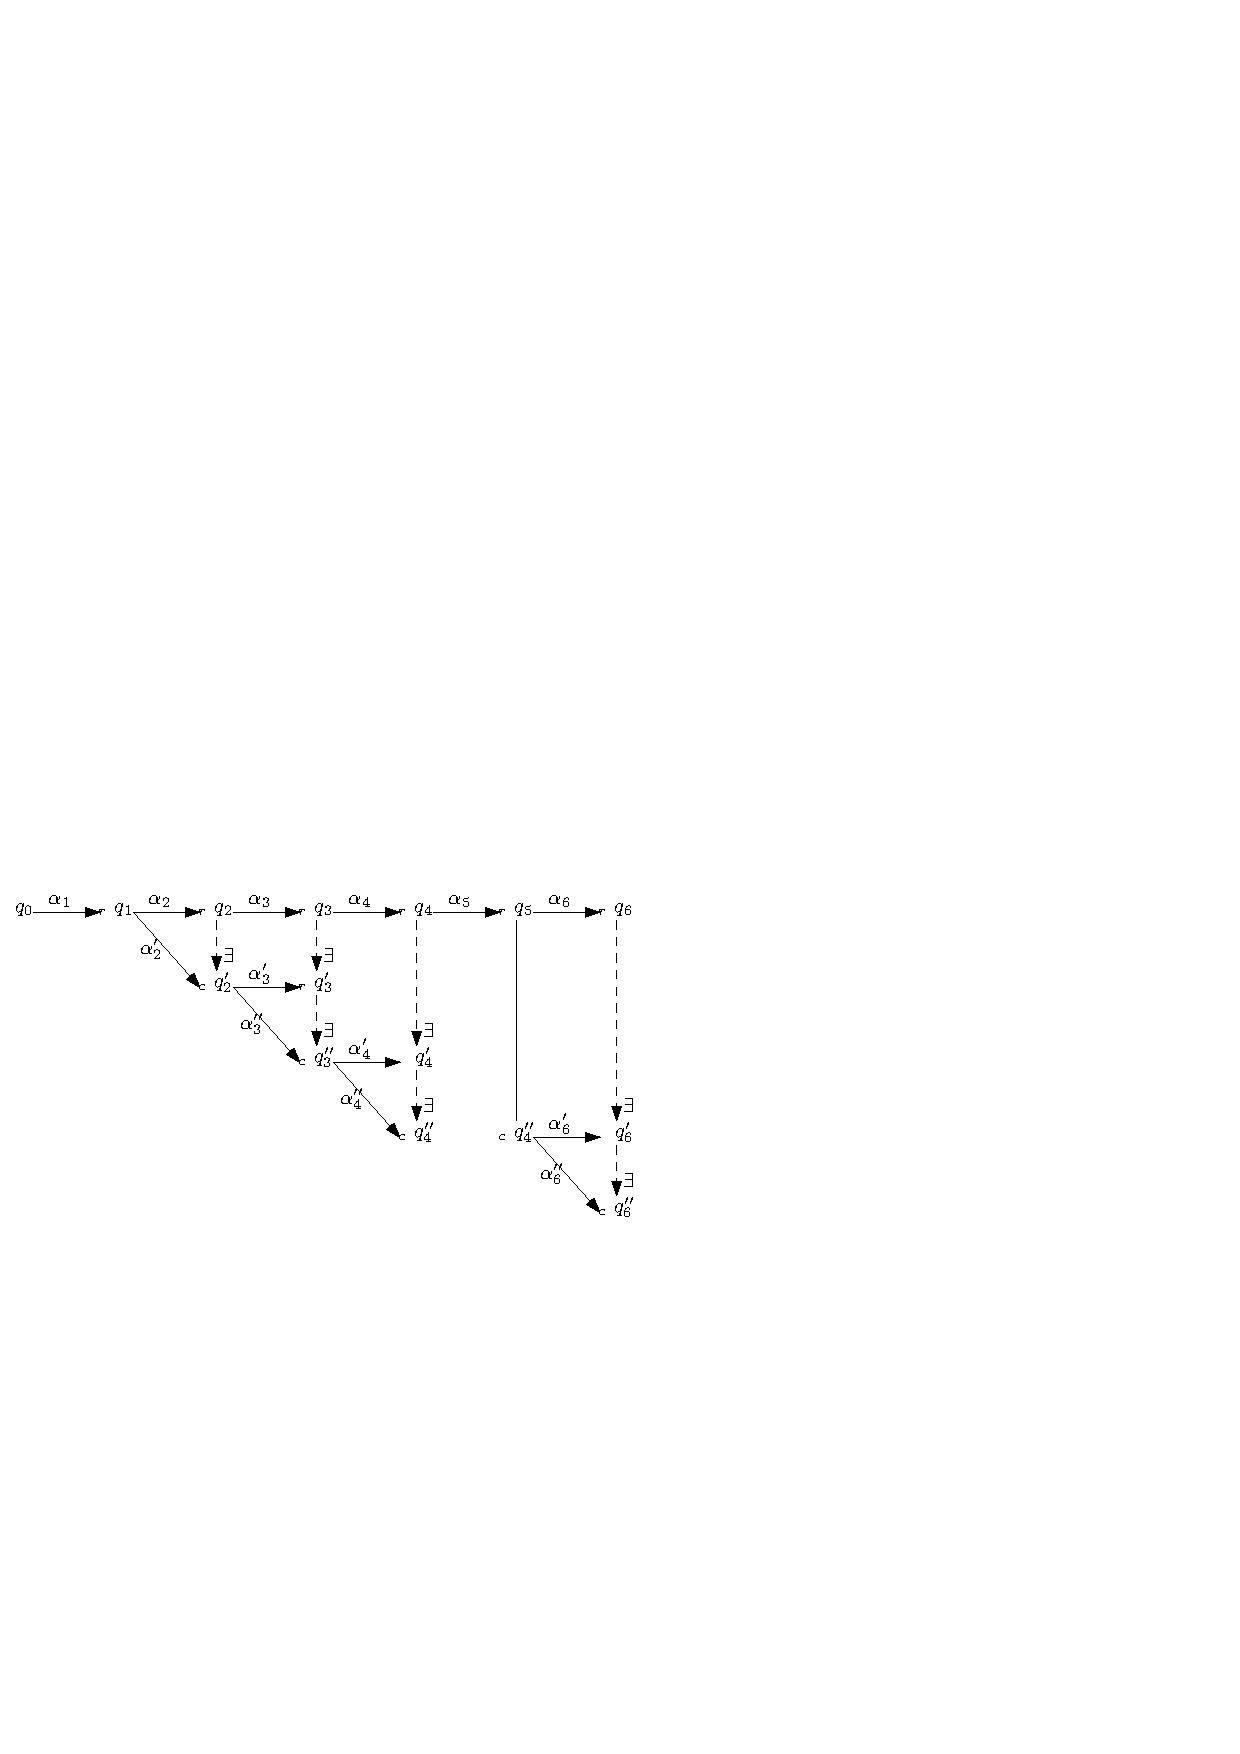
\includegraphics[width=0.6 \textwidth]{figures/PIC-Generate-AbstractTrace-NormaltoCompact.pdf}
%\vspace{-10pt}
%  \caption{The process of generate a trace of $CRImp(Spec)$ from a trace of $RImp(Spec)$}
%  \label{fig:the process of generate a trace of CRImpSpec from a trace of RImpSpec}
%\end{figure}




%{\noindent \bf Lemma \ref{lemma:RIMPSpec and CRIMPSpec have same abstract traces}}: $absT(RImp(Spec)) = absT(CRImp(Spec))$
%\begin {proof}
%The $\supseteq$ direction is obvious from the definition of $absT(CRImp(Spec))$.
%To prove the $\subseteq$ direction. Given a execution $t_1 = \alpha_1 \cdot \ldots \in \llbracket RImp(Spec) \rrbracket$. Let us show how to construct a path of $CRImp(Spec)$.
%\begin{itemize}
%\setlength{\itemsep}{0.5pt}
%\item[-] $q_1 {\xrightarrow{\alpha_2}}_r q_2$: By definition of $\rightarrow_c$, $\exists \alpha'_2$, such that $q_1 {\xrightarrow{\alpha'_2}}_c q'_2 \wedge conc(q_2)=q'_2$. Then, it is obvious that $(q_2,q'_2) \in R_{O_2}$ for some $O_2$.

%\item[-] $q_2 {\xrightarrow{\alpha_3}}_r q_3$: Since $(q_2,q'_2) \in R_{O_2} \wedge q_2 {\xrightarrow{\alpha_3}}_r q_3 $, we can see that $\exists \alpha'_3,q'_3$, such that $q'_2 {\xrightarrow{\alpha'_3}}_r q'_3 \wedge (q_3,q'_3) \in R_{O_2}$.

    %By definition of $\rightarrow_c$, $\exists \alpha''_3$, such that $q'_2 {\xrightarrow{\alpha''_3}}_c q''_3 \wedge conc(q'_3)=q''_3$. Then, it is obvious that $(q'_3,q''_3) \in R_{O_3}$ for some $O_3$. Therefore, $(q_3,q''_3) \in R_{(O_2 \cup O_3)}$.

%\item[-] If $i \geq 3 \wedge q_i {\xrightarrow{addDel(o,r)}}_r q_{i+1} \wedge o \in S_p(q_i) \cup S_m(q_i)$: We already know that $(q_i,q''_i) \in R_{O}$ for some $O$, then it is obvious that $(q_{i+1},q''_{i+1}) \in R_{O}$, where $q''_{i+1} = q''_i$.

%\item[-] If $i \geq 3 \wedge q_i {\xrightarrow{\alpha_{i+1}}}_r q_{i+1} \neg (\alpha_i = addDel(o,r) \wedge o \in S_p(q_i) \cup S_m(q_i))$: We already know that $(q_i,q''_i) \in R_{O}$ for some $O$. Since $q_i {\xrightarrow{\alpha_{i+1}}}_r q_{i+1}$, we can see that $\exists \alpha'_{i+1},q'_{i+1}$, such that $q''_i {\xrightarrow{\alpha'_{i+1}}}_r q'_{i+1} \wedge (q_{i+1},q'_{i+1}) \in R_{O}$.

    %By definition of $\rightarrow_c$, $\exists \alpha''_{i+1}$, such that $q''_i {\xrightarrow{\alpha''_{i+1}}}_c q''_{i+1} \wedge conc(q'_{i+1})=q''_{i+1}$. Then, it is obvious that $(q'_{i+1},q''_{i+1}) \in R_{O_{i+1}}$ for some $O_{i+1}$. Therefore, $(q_{i+1},q''_{i+1}) \in R_{(O \cup O_{i+1})}$.
%\end{itemize}

%\figurename~\ref{fig:the process of generate a trace of CRImpSpec from a trace of RImpSpec} given an example when (1) $q_0 {\xrightarrow{\alpha_1}}_r q_1 {\xrightarrow{\alpha_2}}_r q_2 {\xrightarrow{\alpha_3}}_r q_3 {\xrightarrow{\alpha_4}}_r q_4 {\xrightarrow{\alpha_5}}_r q_6 {\xrightarrow{\alpha_6}}_r q_6$ is a path of $RImp(Spec)$, (2) $\alpha_5=addDel(o,r) \wedge o \in S_p(q_4) \cup S_m(q_4)$, and $\forall i \neq 5$, $\neg ( \alpha_i=addDel(o,r) \wedge o \in S_p(q_{i-1}) \cup S_m(q_{i-1})$.

%It is easy to see that the abstract trace of $\alpha_1 \cdot \alpha_2 \cdot \alpha_3 \cdot \alpha_4$ in $RImp(Spec)$ is the abstract trace of $\alpha_1 \cdot \alpha'_2 \cdot \alpha''_3 \cdot \alpha''_4$ in $CRImp(Spec)$. This completes the proof of this lemma. $\qed$
%\end {proof}















\section{Definitions and Proofs of Section \ref{sec:implementation}}
\label{sec:appendix definitions and proofs of section implementation}



{\noindent \bf Lemma \ref{lemma:semantics of imp cd contains the set of causal delivery executions of semantics of imp}}: $\llbracket imp \rrbracket_{cd} = \{ t \vert t \in \llbracket imp \rrbracket \wedge t$ satisfies causal delivery $\}$.

\begin {proof}

Given $t = \alpha_1 \cdot \ldots \in \llbracket imp \rrbracket_{cd}$, if there exists $q_1,\ldots \in Q$, such that $q_0 {\xrightarrow{\alpha_1}} q_1 {\xrightarrow{\alpha_2}} \ldots$. We need to prove the following property: On each state $q_i=(repD_i,msgs_i,<_i)$,

\begin{itemize}
\setlength{\itemsep}{0.5pt}
\item[-] $P_1$: $msgs_i = \{ (dat,r,r') \vert$ the operation generating this message is launched by replica $r$ and its message has not been applied to replica $r'$ in $t[1,i]\}$.

\item[-] $P_2$: $m_1 <_i m_2$, iff $m_1$ and $m_2$ have same destination replica, and the operation generating $m_1$ happens before the operation generating $m_2$ in $t[1,i]$.

\item[-] $P_3$: $m <_i r$, iff the destination replica of $m$ is not $r$, and the operation generating $m$ is visible to replica $r$ in $t[1,i]$, and does not happen before ``any operation that launched by replica $r$'' in $t[1,i]$.
\end{itemize}

Once we prove that $P_1$, $P_2$ and $P_3$ holds for each $q_i$, let us prove this lemma by contradiction: Assume that update operations $o_1 <_{hb} o_2$, messages of $o_1$ are $\{ (d_1,r_1,\_) \}$, messages of $o_2$ are \{ $(d_2,r_2,\_) \}$, $\alpha_i = apply((d_2,r_2,r'),r')$, $\alpha_j = apply((d_1,r_1,r'),r')$, and $i<j$. Then in $q_i=(repD_i,msgs_i,<_i)$, since $o_1 <_{hb} o_2$ and transition rules of $\llbracket imp \rrbracket_{cd}$, we could not launch $apply((d_2,r_2,r'),r')$ transition, which is the contradiction.



Let us begin to prove that each state $q_i=(repD_i,msgs_i,<_i)$ satisfies properties $P_1$, $P_2$ and $P_3$. We prove this by induction on $t$.

\begin{itemize}
\setlength{\itemsep}{0.5pt}
\item[-] It is obvious that $q_0$ satisfies properties $P_1$, $P_2$ and $P_3$.

\item[-] Since $\alpha_1$ must be either a query transition or an update transition, it is easy to see that $<_1 = \emptyset$ and $q_1$ satisfies properties $P_1$, $P_2$ and $P_3$.

\item[-] Assume that $q_i=(repD_i,msgs_i,<_i)$ satisfies properties $P_1$, $P_2$ and $P_3$. let us consider $q_{i+1}= (repD_{i+1},msgs_{i+1},<_{i+1})$,

    \begin{itemize}
    \setlength{\itemsep}{0.5pt}
    \item[-] If $q_{i+1}$ is obtained from $q_i$ by a query transition, then this holds obviously.

    \item[-] Else, if $q_{i+1}$ is obtained from $q_i$ by a update transition. Then we can see that $(repD_i,msgs_i,<_i) {\xrightarrow{m(a,b,r)}} (repD_{i+1},msgs_{i+1}=msgs \cup \{ (dat,r,r') \vert  r' \in RId \wedge r \neq r' \},<_{i+1} = <_i \otimes dat)$.

        Since we add messages $\{ (dat,r,r') \vert  r' \in RId \wedge r \neq r' \}$ into $msgs_i$, we can see that $P_1$ holds.

        To satisfy $P_2$ and $P_3$, we need to make newly add messages maximal w.r.t $<$ and still keep transitivity, which is done by $<_i \otimes dat$.

    \item[-] Else, $q_{i+1}$ is obtained from $q_i$ by a applying transition. Then we can see that $(repD_i,msgs_i,<_i) {\xrightarrow{apply(m=(dat,r_1,r))}} (repD_{i+1},msgs_{i+1} = msgs_i - \{ m \}, <_{i+1} = <_i \otimes m )$, where $m$ is minimal w.r.t $<_i$ among messages in $msgs_i(r)$.

        Since we use one message $m$ in this process and remove it from $msgs_i$, we can see that $P_1$ holds.

        Applying message will introduce new visibility relation. To satisfy $P_2$ and $P_3$, we need to first forget $m$, record the newly introduced visibility relation, and still keep transitivity. This is done by $<_i \otimes m$.
    \end{itemize}
\end{itemize}

This completes the proof of this lemma. $\qed$
\end {proof}

















\forget
{
\section{Definitions and Proofs of Section \ref{sec:reference implementation}}
\label{sec:appendix definitions and proofs of section reference implementation}



\subsection{Proof of Lemma \ref{lemma:executions of reference implementation are eventual consistent}}
\label{subsec:appendix proof of lemma executions of reference implementation are eventual consistent}

{\noindent \bf Lemma \ref{lemma:executions of reference implementation are eventual consistent}}: $\forall t \in \llbracket RImp(Spec) \rrbracket$, $poSet(t)$ is eventual consistent w.r.t $Spec$.

\begin {proof}

Assume $RImp(Spec) = (Q,\Sigma,vis,,q_0,li,\rightarrow,livReq)$, let $t = \alpha_1, \ldots, $ and $\exists q_1,\ldots$, such that $q_0 {\xrightarrow{\alpha_1}} q_1 {\xrightarrow{\alpha_2}} \ldots$, and $livReq(t) = \textit{true}$. Let $poSet(t)=(O_t,<_t)$. Let $gi = (O_t,<_{gi})$ be the global interpretation of $t$.

For each operation $o$, assume $o$ is first introduced by a transition from $q_i$ to $q_{i+1}$, then, the local interpretation of $o$ is $li(q_i,r)$, where $r$ is the replica of $o$.

We prove this lemma by consider the four requirements individually:

\begin{itemize}
\setlength{\itemsep}{0.5pt}
\item[-] $\textit{GIpf}$: Let us consider two kinds of operations $o$.

If $\exists o'$, such that $o' <_{gi} o$, then $\exists i < j$, such that $o'$ and $o$ are the operations of $\alpha_i$ and $\alpha_j$, respectively, and one of the following cases holds: (1) $o'$ and $o$ are of same replica, or (2) $\exists i', i < i' < j$, $\alpha_{i'}=addDel(o',r')$ and $r'$ is the replica of $o$. In each case, it is easy to see that $<^{-1}_{gi}(o)$ contains lee or equal operations than the set of operations in $t[1,j]$ and its number is obviously finite.

    If $\neg \exists o'$, such that $o' <_{gi} o$, then it is easy to see that $o$ is the first operation of its replica and no operation is delivered to that replica before $o$. In this case, it is obvious that $<^{-1}_{gi}(o)$ is finite.

\item[-] $\textit{THINAIR}$: According to the definition, we could see that on each state $q_i$, local interpretation is a subset of visibility relation, and $ro$ is also a subset of visibility relation. It is easy to prove that on each state, $vis$ is acyclic.

\item[-] $\textit{RVAL}$: We only need to consider query operations for $\textit{RVAL}$ property, since only query operations have return values. According to construction of $\llbracket RImp(Spec) \rrbracket$, to launch a query operation $(m,a,b,rid,oid)$ transition of replica $r$ from state $q_i$, we already check whether $li(q_i,r)$, the local interpretation w.r.t $q_i$ and $r$, is in $Spec(m,a,b)$.

\item[-] $\textit{EVENTUAL}$: Let $P=(O_P,<_P)$ be a finite prefix of $gi$.

We can see that $<_P$ is the visibility relation of operations in $O_P$. Let $O'_P = \{ o \vert \exists o_1,o_2 \in O_P,$ $o_1$ is visible to $o_2$ via $o'_1,\ldots,o'_m$, and $o \in \{ o'_1,\ldots,o'_n \} \}$. It is easy to see that $O'_P$ is finite, and assume that operations of $O_P \cup O'_P$ are chosen before $\alpha_{idx}$

Since $livReq(t)=true$, $\exists idx1$, such that in $t[1,idx1]$, all operations in $t[1,idx]$ has been delivered to every replica. According to our construction of $li$, this implies that for each state after $\alpha_{idx1}$ and each replica (1) its local interpretation contains $O_P$ and $O'_P$, and (2) the relation of local interpretation then contains the visibility relation between operations in $O_P$.
\end{itemize}

This completes the proof of this lemma. $\qed$
\end {proof}








\section{Definitions and Proofs of Section \ref{sec:implementation}}
\label{sec:appendix definitions and proofs of section implementation}



{\noindent \bf Lemma \ref{lemma:semantics of imp cd contains the set of causal delivery executions of semantics of imp}}: $\llbracket imp \rrbracket_{cd} = \{ t \vert t \in \llbracket imp \rrbracket \wedge t$ satisfies causal delivery $\}$.

\begin {proof}

Given $t = \alpha_1 \cdot \ldots \in \llbracket imp \rrbracket_{cd}$, if there exists $q_1,\ldots \in Q$, such that $q_0 {\xrightarrow{\alpha_1}} q_1 {\xrightarrow{\alpha_2}} \ldots$. We need to prove the following property: On each state $q_i=(repD_i,msgs_i,<_i)$,

\begin{itemize}
\setlength{\itemsep}{0.5pt}
\item[-] $P_1$: $msgs_i = \{ (dat,r,r') \vert$ the operation generating this message is launched by replica $r$ and its message has not been applied to replica $r'$ in $t[1,i]\}$.

\item[-] $P_2$: $m_1 <_i m_2$, iff $m_1$ and $m_2$ have same destination replica, and the operation generating $m_1$ happens before the operation generating $m_2$ in $t[1,i]$.

\item[-] $P_3$: $m <_i r$, iff the destination replica of $m$ is not $r$, and the operation generating $m$ is visible to replica $r$ in $t[1,i]$, and does not happen before ``any operation that launched by replica $r$'' in $t[1,i]$.
\end{itemize}

Once we prove that $P_1$, $P_2$ and $P_3$ holds for each $q_i$, let us prove this lemma by contradiction: Assume that update operations $o_1 <_{hb} o_2$, messages of $o_1$ are $\{ (d_1,r_1,\_) \}$, messages of $o_2$ are \{ $(d_2,r_2,\_) \}$, $\alpha_i = apply((d_2,r_2,r'),r')$, $\alpha_j = apply((d_1,r_1,r'),r')$, and $i<j$. Then in $q_i=(repD_i,msgs_i,<_i)$, since $o_1 <_{hb} o_2$ and transition rules of $\llbracket imp \rrbracket_{cd}$, we could not launch $apply((d_2,r_2,r'),r')$ transition, which is the contradiction.



Let us begin to prove that each state $q_i=(repD_i,msgs_i,<_i)$ satisfies properties $P_1$, $P_2$ and $P_3$. We prove this by induction on $t$.

\begin{itemize}
\setlength{\itemsep}{0.5pt}
\item[-] It is obvious that $q_0$ satisfies properties $P_1$, $P_2$ and $P_3$.

\item[-] Since $\alpha_1$ must be either a query transition or an update transition, it is easy to see that $<_1 = \emptyset$ and $q_1$ satisfies properties $P_1$, $P_2$ and $P_3$.

\item[-] Assume that $q_i=(repD_i,msgs_i,<_i)$ satisfies properties $P_1$, $P_2$ and $P_3$. let us consider $q_{i+1}= (repD_{i+1},msgs_{i+1},<_{i+1})$,

    \begin{itemize}
    \setlength{\itemsep}{0.5pt}
    \item[-] If $q_{i+1}$ is obtained from $q_i$ by a query transition, then this holds obviously.

    \item[-] Else, if $q_{i+1}$ is obtained from $q_i$ by a update transition. Then we can see that $(repD_i,msgs_i,<_i) {\xrightarrow{m(a,b,r)}} (repD_{i+1},msgs_{i+1}=msgs \cup \{ (dat,r,r') \vert  r' \in RId \wedge r \neq r' \},<_{i+1} = <_i \otimes dat)$.

        Since we add messages $\{ (dat,r,r') \vert  r' \in RId \wedge r \neq r' \}$ into $msgs_i$, we can see that $P_1$ holds.

        To satisfy $P_2$ and $P_3$, we need to make newly add messages maximal w.r.t $<$ and still keep transitivity, which is done by $<_i \otimes dat$.

    \item[-] Else, $q_{i+1}$ is obtained from $q_i$ by a applying transition. Then we can see that $(repD_i,msgs_i,<_i) {\xrightarrow{apply(m=(dat,r_1,r))}} (repD_{i+1},msgs_{i+1} = msgs_i - \{ m \}, <_{i+1} = <_i \otimes m )$, where $m$ is minimal w.r.t $<_i$ among messages in $msgs_i(r)$.

        Since we use one message $m$ in this process and remove it from $msgs_i$, we can see that $P_1$ holds.

        Applying message will introduce new visibility relation. To satisfy $P_2$ and $P_3$, we need to first forget $m$, record the newly introduced visibility relation, and still keep transitivity. This is done by $<_i \otimes m$.
    \end{itemize}
\end{itemize}

This completes the proof of this lemma. $\qed$
\end {proof}
}












\end{document}








